\chapter{Analyse \& Conception}

\section{Introduction}
Le but de ce chapitre est d'aborder les concepts essentiels a la réalisation du projet.\\

En première partie, nous ferons un rappel sur les généralités d'UML, sa définition et ses diagrammes.\\

Par la suite, nous passerons à l'analyse des principaux utilisateurs du système et les besoins de ces derniers.\\

Nous terminerons par une conception des diagrammes de classes et des diagrammes de séquences ainsi qu'une présentation de la structure de la base de données.\\

\section{Présentation d'\acs{UML}}
\acs{UML}\cite{uml-diag} est un acronym qui signifie Unified Modeling Langage ou Langage de Modélisation Unifié en français, est apparu pour la première fois dans les années 1990. En simple, \acs{UML} est une approche moderne et méthodique de la modélisation et de la documentation des applications. C'est l'une des techniques de modélisation des processus d'entreprise les plus populaires.\\

Son approche est basée sur des représentations schématiques des composants d'un logiciel. Cette représentations visuelles nous donnent la possibilité de mieux mesurer les éventuelles erreurs ou défauts des logiciels.\\

\subsection{Les diagrammes \acs{UML}}
La représentation graphique des composants d'un logiciel\cite{uml-diag} et faites à l'aide de diagrammes. Ces diagrammes sont simples, stricte et contiennent des règles d'utilisations et de syntaxes bien fix.\\

UML nous permet d'établir une représentation du logiciel sous plusieurs angles ou vues:

\begin{itemize}
    \item \textbf{Vue des cas d’utilisation} : vue des acteurs (besoins attendus)
    \item \textbf{Vue logique} : vue de l'intérieur (satisfaction des besoins)
    \item \textbf{Vue d’implantation} : dépendances entre les modules
    \item \textbf{Vue des processus} : dynamique du système
    \item \textbf{Vue de déploiement} : organisation environnementale du logiciel
\end{itemize}

UML est composé de plusieurs diagrammes chacun d'eux sert à des objectifs différent qu'il soit avant ou après la mise en oeuvre.

\section{Analyse}
La phase d’analyse débute par l'identification des acteurs ainsi que leurs différentes tâches dans le système, ensuite, la spécification des besoins fonctionnels et non fonctionelles du système. Ceci nous mène vers une schématisation par un diagramme des cas d’utilisation traduisant la dynamique système qui sera utilisé dans la phase de conception.


\subsection{Spécification des besoins}
\subsubsection{Besoins fonctionnels}
C’est une description des caractéristiques du système et de ses fonctionnalités. En partant de ce principe notre application doit permettre :\\

    \textbf{Visiteurs\\}
        \textbf{Consultation de la page d’accueil}
        \begin{itemize}
            \item Consulter le service d'hébergements
            \item Télécharger le document d'aide à la constitution du dossier d'hébergement
            \item Consulter le service de restauration
            \item Consulter le service des transports
            \item Consulter le service des bourses
            \item Télécharger le document d'aide à la constitution du dossier de bourse
            \item Télécharger le document d'aide au renouvellement du dossier de bourse
            \item Télécharger le document d'aide au transfert du dossier de bourse\\
        \end{itemize}

        \textbf{Consultation du calendrier des menus de chaque restaurant d'un mois défini}
        \begin{itemize}
            \item Changer le mois du calendrier des menus
            \item Changer l'affichage des menus par mois, semaine, jour de travail, jour et par agenda
            \item Voir plus d'informations sur un seul menu\\
        \end{itemize} 
        
        \textbf{Consultation du calendrier de tous les trajets de chaque Campus/Résidence d'un mois défini}
        \begin{itemize}
            \item Changer le mois du calendrier des trajets
            \item Changer l’affichage des trajets par mois, semaine, jour de travail, jour et par agenda
            \item Voir plus de détails sur un seul trajet \\
        \end{itemize}

\textbf{Staff\\}
En plus des fonctionnalités du visiteur le staff peut aussi:\\

    \textbf{Hébergement}
    \begin{itemize}
        \item Consulter la liste des dossiers d'hébergement
        \item Sélectionner un ou plusieurs dossiers d'hébergement
        \item Ajouter un dossier d'hébergement
        \item Supprimer un ou plusieurs dossier(s) d'hébergement
        \item Voir plus d'informations sur un dossier d'hébergement
        \item Valider un dossier d'hébergement
        \item Refuser un dossier d'hébergement \\
    \end{itemize}

    \textbf{Bourse}
    \begin{itemize}
        \item Consulter la liste des dossiers de bourse
        \item Sélectionner un ou plusieurs dossiers de bourse
        \item Ajouter un dossier de bourse
        \item Supprimer un ou plusieurs dossier(s) de bourse
        \item Voir plus d'informations sur un dossier de bourse
        \item Valider un dossier de bourse
        \item Refuser un dossier de bourse
        \item Changer l'ordre d'affichage par attributs \\
    \end{itemize}

    \textbf{Campus \& Résidences}
    \begin{itemize}
        \item Consulter la liste des Campus \& Résidences
        \item Ajouter un campus ou une résidence
        \item Supprimer un campus ou une résidence
        \item Voir plus d'informations sur un campus ou une résidence
        \item Modifier les informations d'un campus ou une résidence
        \item Rechercher un campus ou une résidence
        \item Filtrer par campus seulement résidences seulement ou par campus \& résidences \\
    \end{itemize}

    \textbf{Transport - Calendrier}
    \begin{itemize}
        \item Voir les trajets détaillé de tout le mois
        \item Ajouter un trajet
        \item Modifier un trajet
        \item Supprimer un trajet \\
    \end{itemize}

    \textbf{Transport - Bus}
    \begin{itemize}
        \item Consulter la liste des bus
        \item Sélectionner un ou plusieurs bus
        \item Ajouter un bus
        \item Supprimer un ou plusieurs bus
        \item Voir plus d'informations sur un bus
        \item Modifier les informations d'un bus
        \item Filtrer par attributs \\
    \end{itemize}

    \textbf{Restauration - Calendrier}
    \begin{itemize}
        \item Voir les menus détaillé de tout le mois par semaine
        \item Ajouter un menu
        \item Modifier un menu
        \item Supprimer un menu \\
    \end{itemize}

    \textbf{Restauration - Restaurants}
    \begin{itemize}
        \item Consulter la liste des restaurants
        \item Ajouter un restaurant
        \item Supprimer un restaurant
        \item Voir plus d'informations sur un restaurant
        \item Modifier les informations d'un restaurant
        \item Rechercher un restaurant
        \item Filtrer par les restaurants par établissements ( appartiennent à un campus ou une résidence )\\
    \end{itemize}

    \textbf{Restauration - Plats \& Desserts}
    \begin{itemize}
        \item Consulter la liste des plats \& desserts
        \item Ajouter un plat/dessert
        \item Supprimer un plat/dessert
        \item Voir plus d'informations sur un plat/dessert
        \item Modifier les informations d'un plat/dessert
        \item Rechercher un plat/dessert
        \item Filtrer par plats seulement desserts seulement ou par plats \& desserts\\
    \end{itemize}

    \textbf{Restauration - Ingrédients}
    \begin{itemize}
        \item Consulter la liste des ingrédients
        \item Sélectionner un ou plusieurs ingrédient(s)
        \item Ajouter un ingrédient
        \item Supprimer un ou plusieurs ingrédient(s)
        \item Voir plus d'informations sur un ingrédient
        \item Modifier les informations d'un ingrédient
        \item Filtrer par attribut\\
    \end{itemize}

    \textbf{Administrateur\\}
    En plus des fonctionnalités de l'utilisateur l'administrateur peut aussi: \\
    \textbf{Utilisateurs}
    \begin{itemize}
        \item Consulter la liste des utilisateurs
        \item Sélectionner un ou plusieurs utilisateur(s)
        \item Ajouter un utilisateur
        \item Supprimer un ou plusieurs utilisateur(s)
        \item Voir plus d'informations sur un utilisateur
        \item Modifier les informations d'un utilisateur
        \item Filtrer par attributs\\
    \end{itemize}

\subsubsection{Besoins non fonctionnels}
Ça représente des exigences qui ne concernent pas le comportement du système. Elles identifient les contraintes internes et externes du système. Dans notre cas l’application devra respecter les exigences suivantes :\\

\noindent \textbf{Performance:} temps de réponse petit.\\
\textbf{Maintenabilité:} apporter des corrections facilement.\\
\textbf{Fiabilité:} précise et correcte.\\
\textbf{Intégrabilité:} intégrer de nouvelles fonctionnalités facilement.\\
\textbf{Portabilité:} elle peut fonctionner sur plusieurs plateformes.\\
\textbf{Disponibilité:} réaliser une fonction requise à tout moment.\\
\textbf{Sécurité:} personnaliser les accès selon l’utilisateur.\\

\subsection{Identification des acteurs}
Un acteur est une entité externe qui a la possibilité d'interagir et d'utiliser les multiples fonctionnalités du système.

\subsubsection{Les acteurs qui interviennent dans notre système}
\begin{itemize}
    \item \textbf{L’administrateur :} C’est le cerveau de l’application, il gère toutes les fonctions de l’application ainsi que les utilisateurs et leurs rôles dans le site.
    \item \textbf{L'utilisateur/staff :} Un staff est un gérant, il a un accès global aux fonctions de l'application hormis les fonctions liées aux utilisateurs.
    \item \textbf{Le visiteur :} il peut uniquement consulter le contenu du site.
\end{itemize}

\subsubsection{Diagramme de contexte}
Le diagramme de contexte, comme son nom l'indique, nous permet de bien comprendre de contexte de notre application et des acteurs qui y participent. Il nous permet d'avoir une vue globale sur les utilisateurs du système:

\begin{figure}[H]
    \centering
    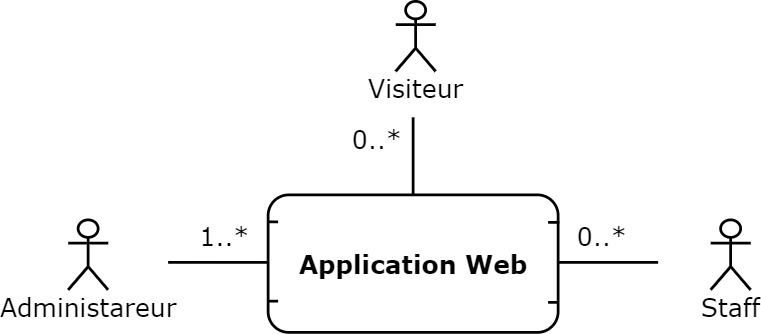
\includegraphics[scale=0.5]{ACR/Diagrammes/contexte.jpg}
    \caption{Diagramme de contexte}
\end{figure}

\subsection{Spécification des tâches}
Dans ce point, nous allons spécifier les tâches de chaque acteur. Le tableau suivant résume ces tâches :

\begin{longtable}{|Z{3cm}|L{10cm}|}
    \caption{Spécification des tâches liées à chaque acteur}\\
    \hline
    \textbf{Acteur} & \textbf{Tâches} \\
    \hline
    \endfirsthead
    \multicolumn{2}{c}%
    {\tablename\ \thetable\ -- \textit{(Suite) Spécification des tâches liées à chaque acteur}} \\
    \hline
    \textbf{Acteur} & \textbf{Tâches} \\
    \hline
    \endhead
    \hline \multicolumn{2}{r}{\textit{(À suivre) Spécification des tâches liées à chaque acteur}} \\
    \endfoot
    \hline
    \endlastfoot
    Visiteurs &
        \textbf{T01 - Consultation de la page d’accueil}
        \begin{itemize}
            \item Consulter le service d'hébergements
            \item Télécharger le document d'aide à la constitution du dossier d'hébergement
            \item Consulter le service de restauration
            \item Consulter le service des transports
            \item Consulter le service des bourses
            \item Télécharger le document d'aide à la constitution du dossier de bourse
            \item Télécharger le document d'aide au renouvellement du dossier de bourse
            \item Télécharger le document d'aide au transfert du dossier de bourse
        \end{itemize} \\
        &
        \textbf{T02 - Consultation du calendrier des menus de chaque restaurant d'un mois défini}
        \begin{itemize}
            \item Changer le mois du calendrier des menus
            \item Changer l'affichage des menus par mois, semaine, jour de travail, jour et par agenda
            \item Voir plus d'informations sur un seul menu
        \end{itemize} \\
        &
        \textbf{T03 - Consultation du calendrier de tous les trajets de chaque Campus/Résidence d'un mois défini}
        \begin{itemize}
            \item Changer le mois du calendrier des trajets
            \item Changer l’affichage des trajets par mois, semaine, jour de travail, jour et par agenda
            \item Voir plus de détails sur un seul trajet
        \end{itemize}
     \\
     \hline
    & \\ &
    En plus des fonctionnalités du visiteur le staff peut aussi:\\
    Staff &
    \textbf{T01 - Hébergement}
    \begin{itemize}
        \item Consulter la liste des dossiers d'hébergement
        \item Sélectionner un ou plusieurs dossiers d'hébergement
        \item Ajouter un dossier d'hébergement
        \item Supprimer un ou plusieurs dossier(s) d'hébergement
    \end{itemize}\\
    &
    \begin{itemize}
        \item Voir plus d'informations sur un dossier d'hébergement
        \item Valider un dossier d'hébergement
        \item Refuser un dossier d'hébergement
    \end{itemize}\\
    &
    \textbf{T02 - Bourse}
    \begin{itemize}
        \item Consulter la liste des dossiers de bourse
        \item Sélectionner un ou plusieurs dossiers de bourse
        \item Ajouter un dossier de bourse
        \item Supprimer un ou plusieurs dossier(s) de bourse
        \item Voir plus d'informations sur un dossier de bourse
        \item Valider un dossier de bourse
        \item Refuser un dossier de bourse
        \item Changer l'ordre d'affichage par attributs
    \end{itemize}\\ &
    \textbf{T03 - Campus \& Résidences}
    \begin{itemize}
        \item Consulter la liste des Campus \& Résidences
        \item Ajouter un campus ou une résidence
        \item Supprimer un campus ou une résidence
        \item Voir plus d'informations sur un campus ou une résidence
        \item Modifier les informations d'un campus ou une résidence
        \item Rechercher un campus ou une résidence
        \item Filtrer par campus seulement résidences seulement ou par campus \& résidences
    \end{itemize}\\
    &
    \textbf{T04 - Transport - Calendrier}
    \begin{itemize}
        \item Voir les trajets détaillé de tout le mois
        \item Ajouter un trajet
        \item Modifier un trajet
        \item Supprimer un trajet
    \end{itemize}\\
    &
    \textbf{T05 - Transport - Bus}
    \begin{itemize}
        \item Consulter la liste des bus
        \item Sélectionner un ou plusieurs bus
        \item Ajouter un bus
        \item Supprimer un ou plusieurs bus
        \item Voir plus d'informations sur un bus
        \item Modifier les informations d'un bus
        \item Filtrer par attributs
    \end{itemize}\\
    &
    \textbf{T06 - Restauration - Calendrier}
    \begin{itemize}
        \item Voir les menus détaillé de tout le mois par semaine
        \item Ajouter un menu
        \item Modifier un menu
        \item Supprimer un menu
    \end{itemize}\\ &
    \textbf{T07 - Restauration - Restaurants}
    \begin{itemize}
        \item Consulter la liste des restaurants
        \item Ajouter un restaurant
        \item Supprimer un restaurant
        \item Voir plus d'informations sur un restaurant
        \item Modifier les informations d'un restaurant
        \item Rechercher un restaurant
        \item Filtrer par les restaurants par établissements ( appartiennent à un campus ou une résidence )
    \end{itemize}\\
    &
    \textbf{T08 - Restauration - Plats \& Desserts}
    \begin{itemize}
        \item Consulter la liste des plats \& desserts
        \item Ajouter un plat/dessert
        \item Supprimer un plat/dessert
        \item Voir plus d'informations sur un plat/dessert
        \item Modifier les informations d'un plat/dessert
        \item Rechercher un plat/dessert
        \item Filtrer par plats seulement desserts seulement ou par plats \& desserts
    \end{itemize}\\
    &
    \textbf{T09 - Restauration - Ingrédients}
    \begin{itemize}
        \item Consulter la liste des ingrédients
        \item Sélectionner un ou plusieurs ingrédient(s)
        \item Ajouter un ingrédient
        \item Supprimer un ou plusieurs ingrédient(s)
        \item Voir plus d'informations sur un ingrédient
        \item Modifier les informations d'un ingrédient
        \item Filtrer par attribut
    \end{itemize} \\
    \hline & \\ Administrateur & 
    En plus des fonctionnalités de l'utilisateur l'administrateur peut aussi:\\
    & \\ &
    \textbf{T01 - Utilisateurs}
    \begin{itemize}
        \item Consulter la liste des utilisateurs
        \item Sélectionner un ou plusieurs utilisateur(s)
        \item Ajouter un utilisateur
        \item Supprimer un ou plusieurs utilisateur(s)
        \item Voir plus d'informations sur un utilisateur
        \item Modifier les informations d'un utilisateur
        \item Filtrer par attributs
    \end{itemize}
\end{longtable}

\subsection{Représentation des diagrammes des cas d'utilisation}
Il répond à la question "Comment les participants au système interagissent-ils avec lui ?". En d'autres termes, le diagramme de cas d'utilisation permet de définir la relation entre le système et les participants.

\subsubsection{Diagramme des cas d’utilisation global}
\paragraph*{Remarque} Les cas d'utilisation de l'acteur "staff" sont nombreux, pour ceux et pour ne pas encombré le diagramme des cas d'utilisation global, nous avons omis les détails de cette acteur puis détaillées, plus bas, les cas d'utilisation spécifiques. \textbf{Les cas dont les détails son omis sont marqué par un asterics "*"}\\

\begin{figure}[H]
    \centering
    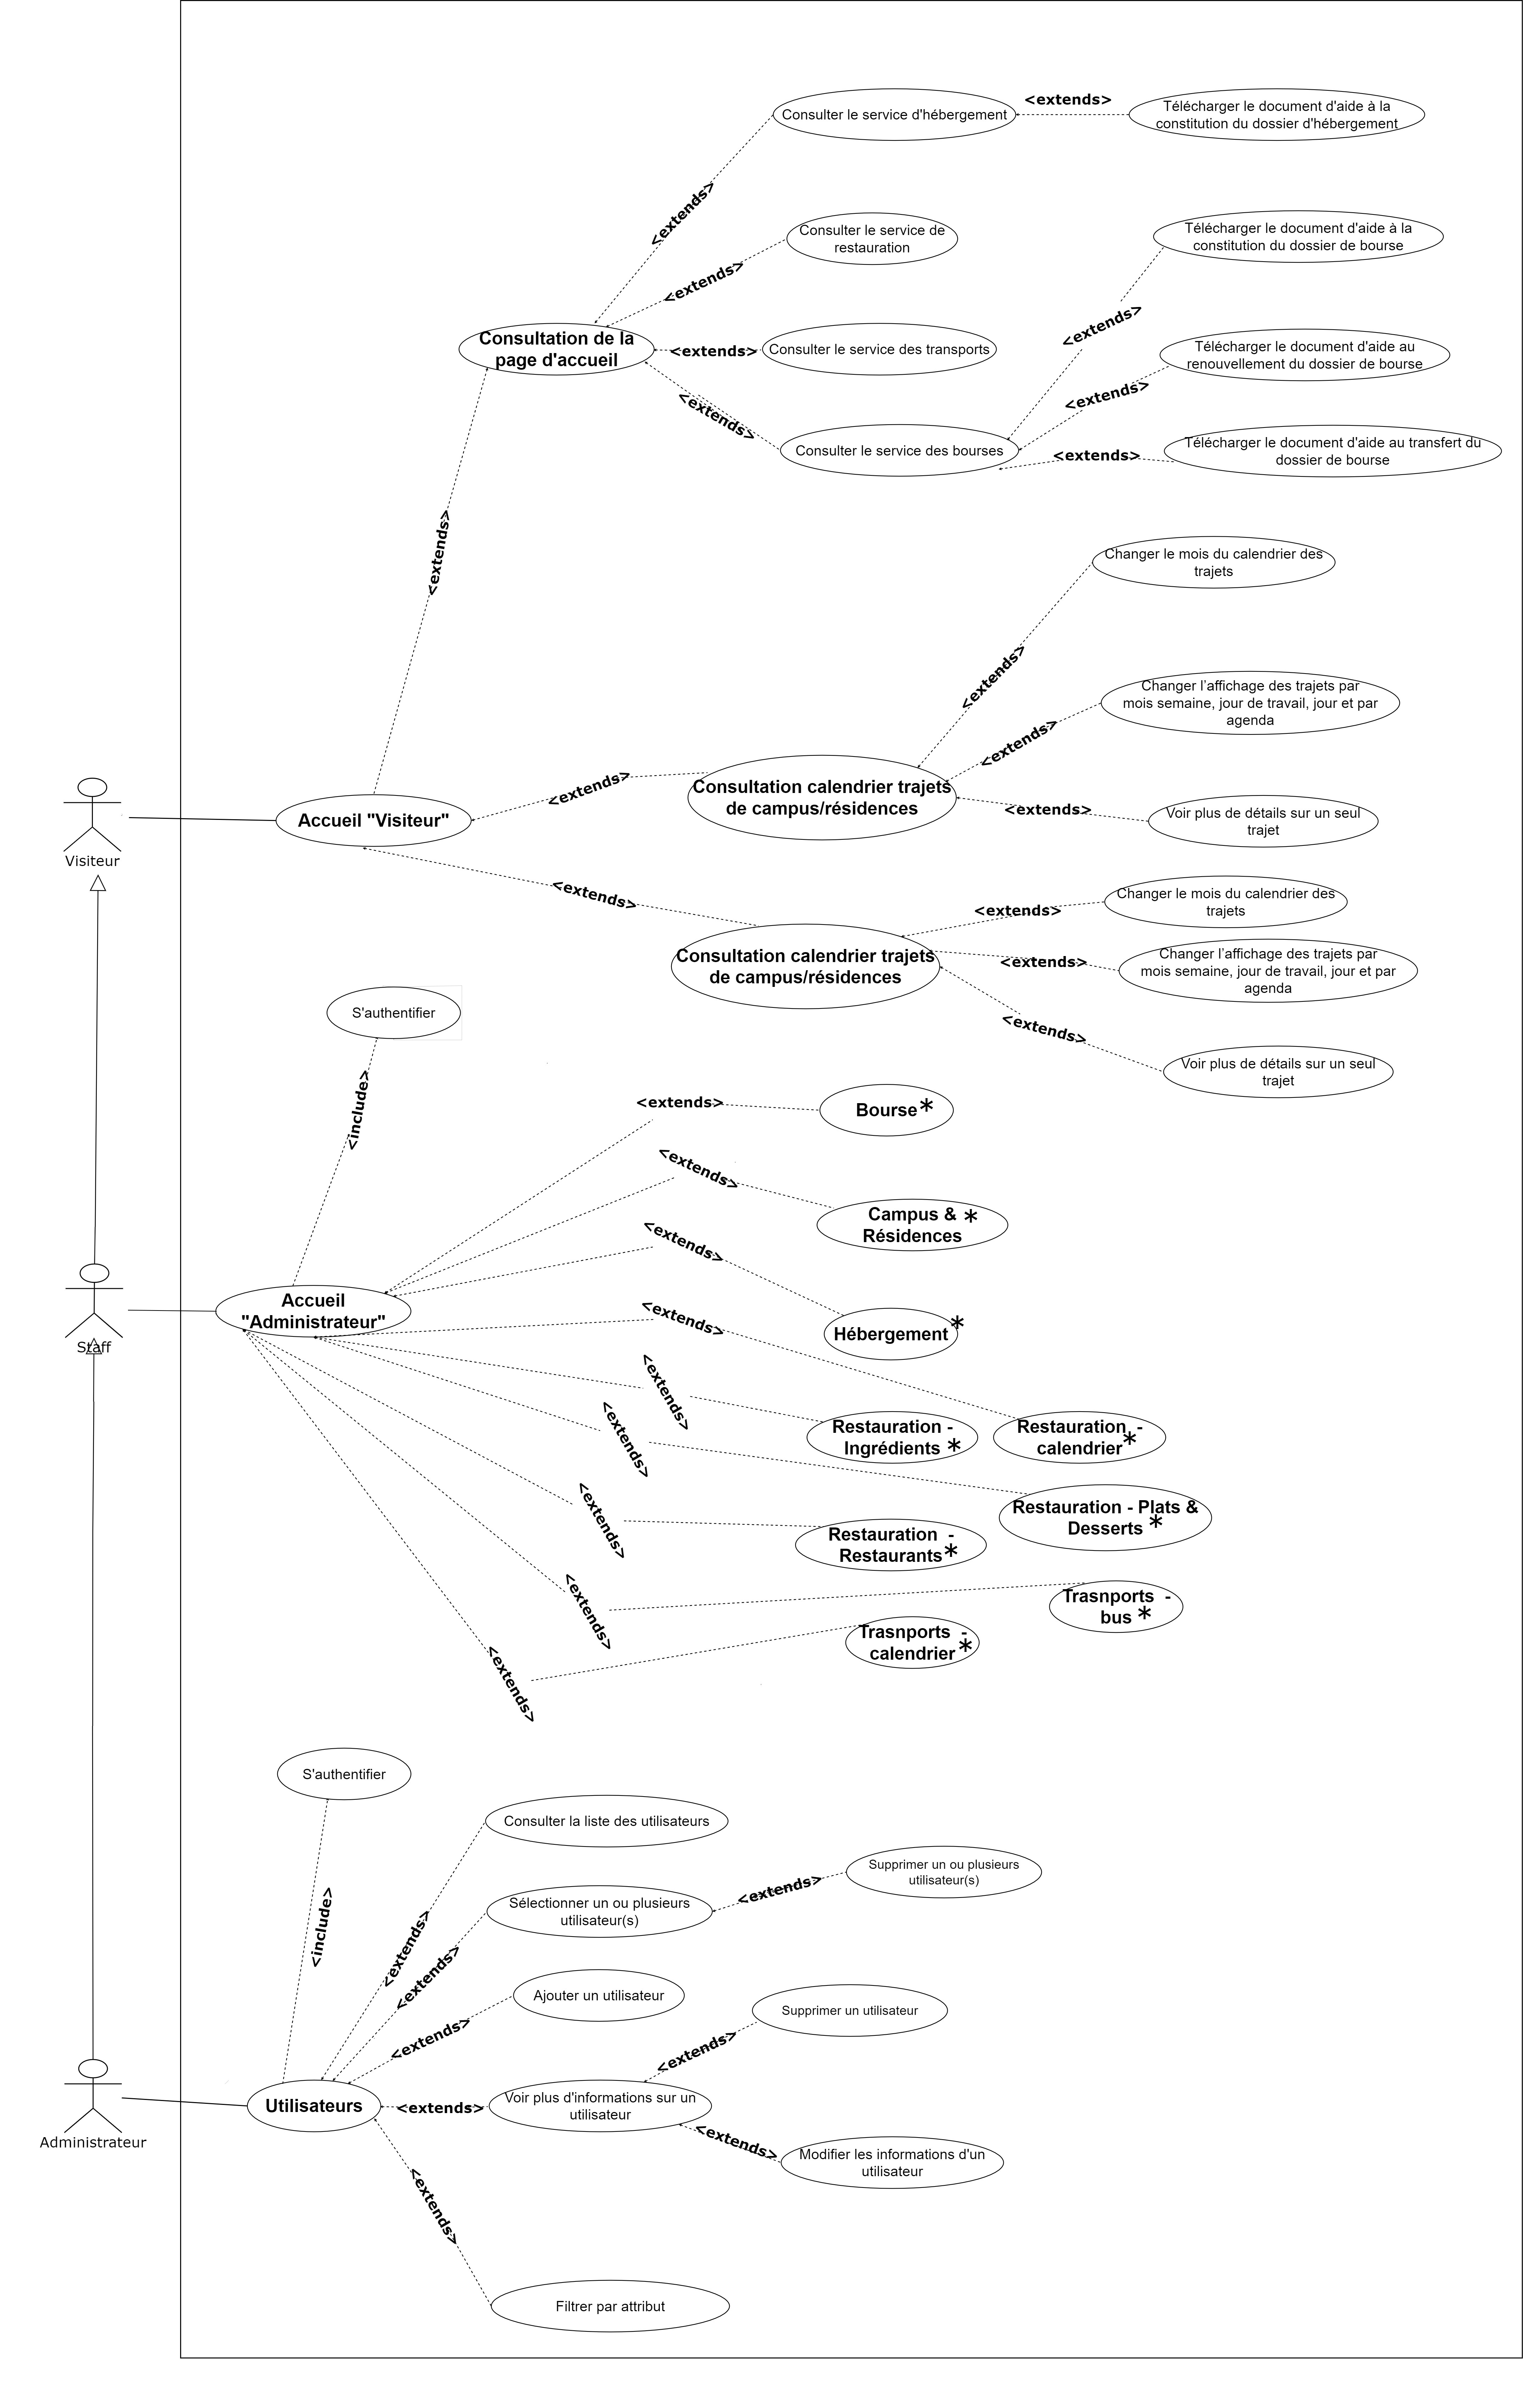
\includegraphics[scale=0.1]{ACR/Diagrammes/Global (1).jpg}
    \caption{Cas d'utilisation global}
\end{figure}

\subsubsection{Diagrammes des cas d’utilisation détaillés}

\subsubsection*{Cas d'utilisation 'Bourses'}
\begin{figure}[H]
    \centering
    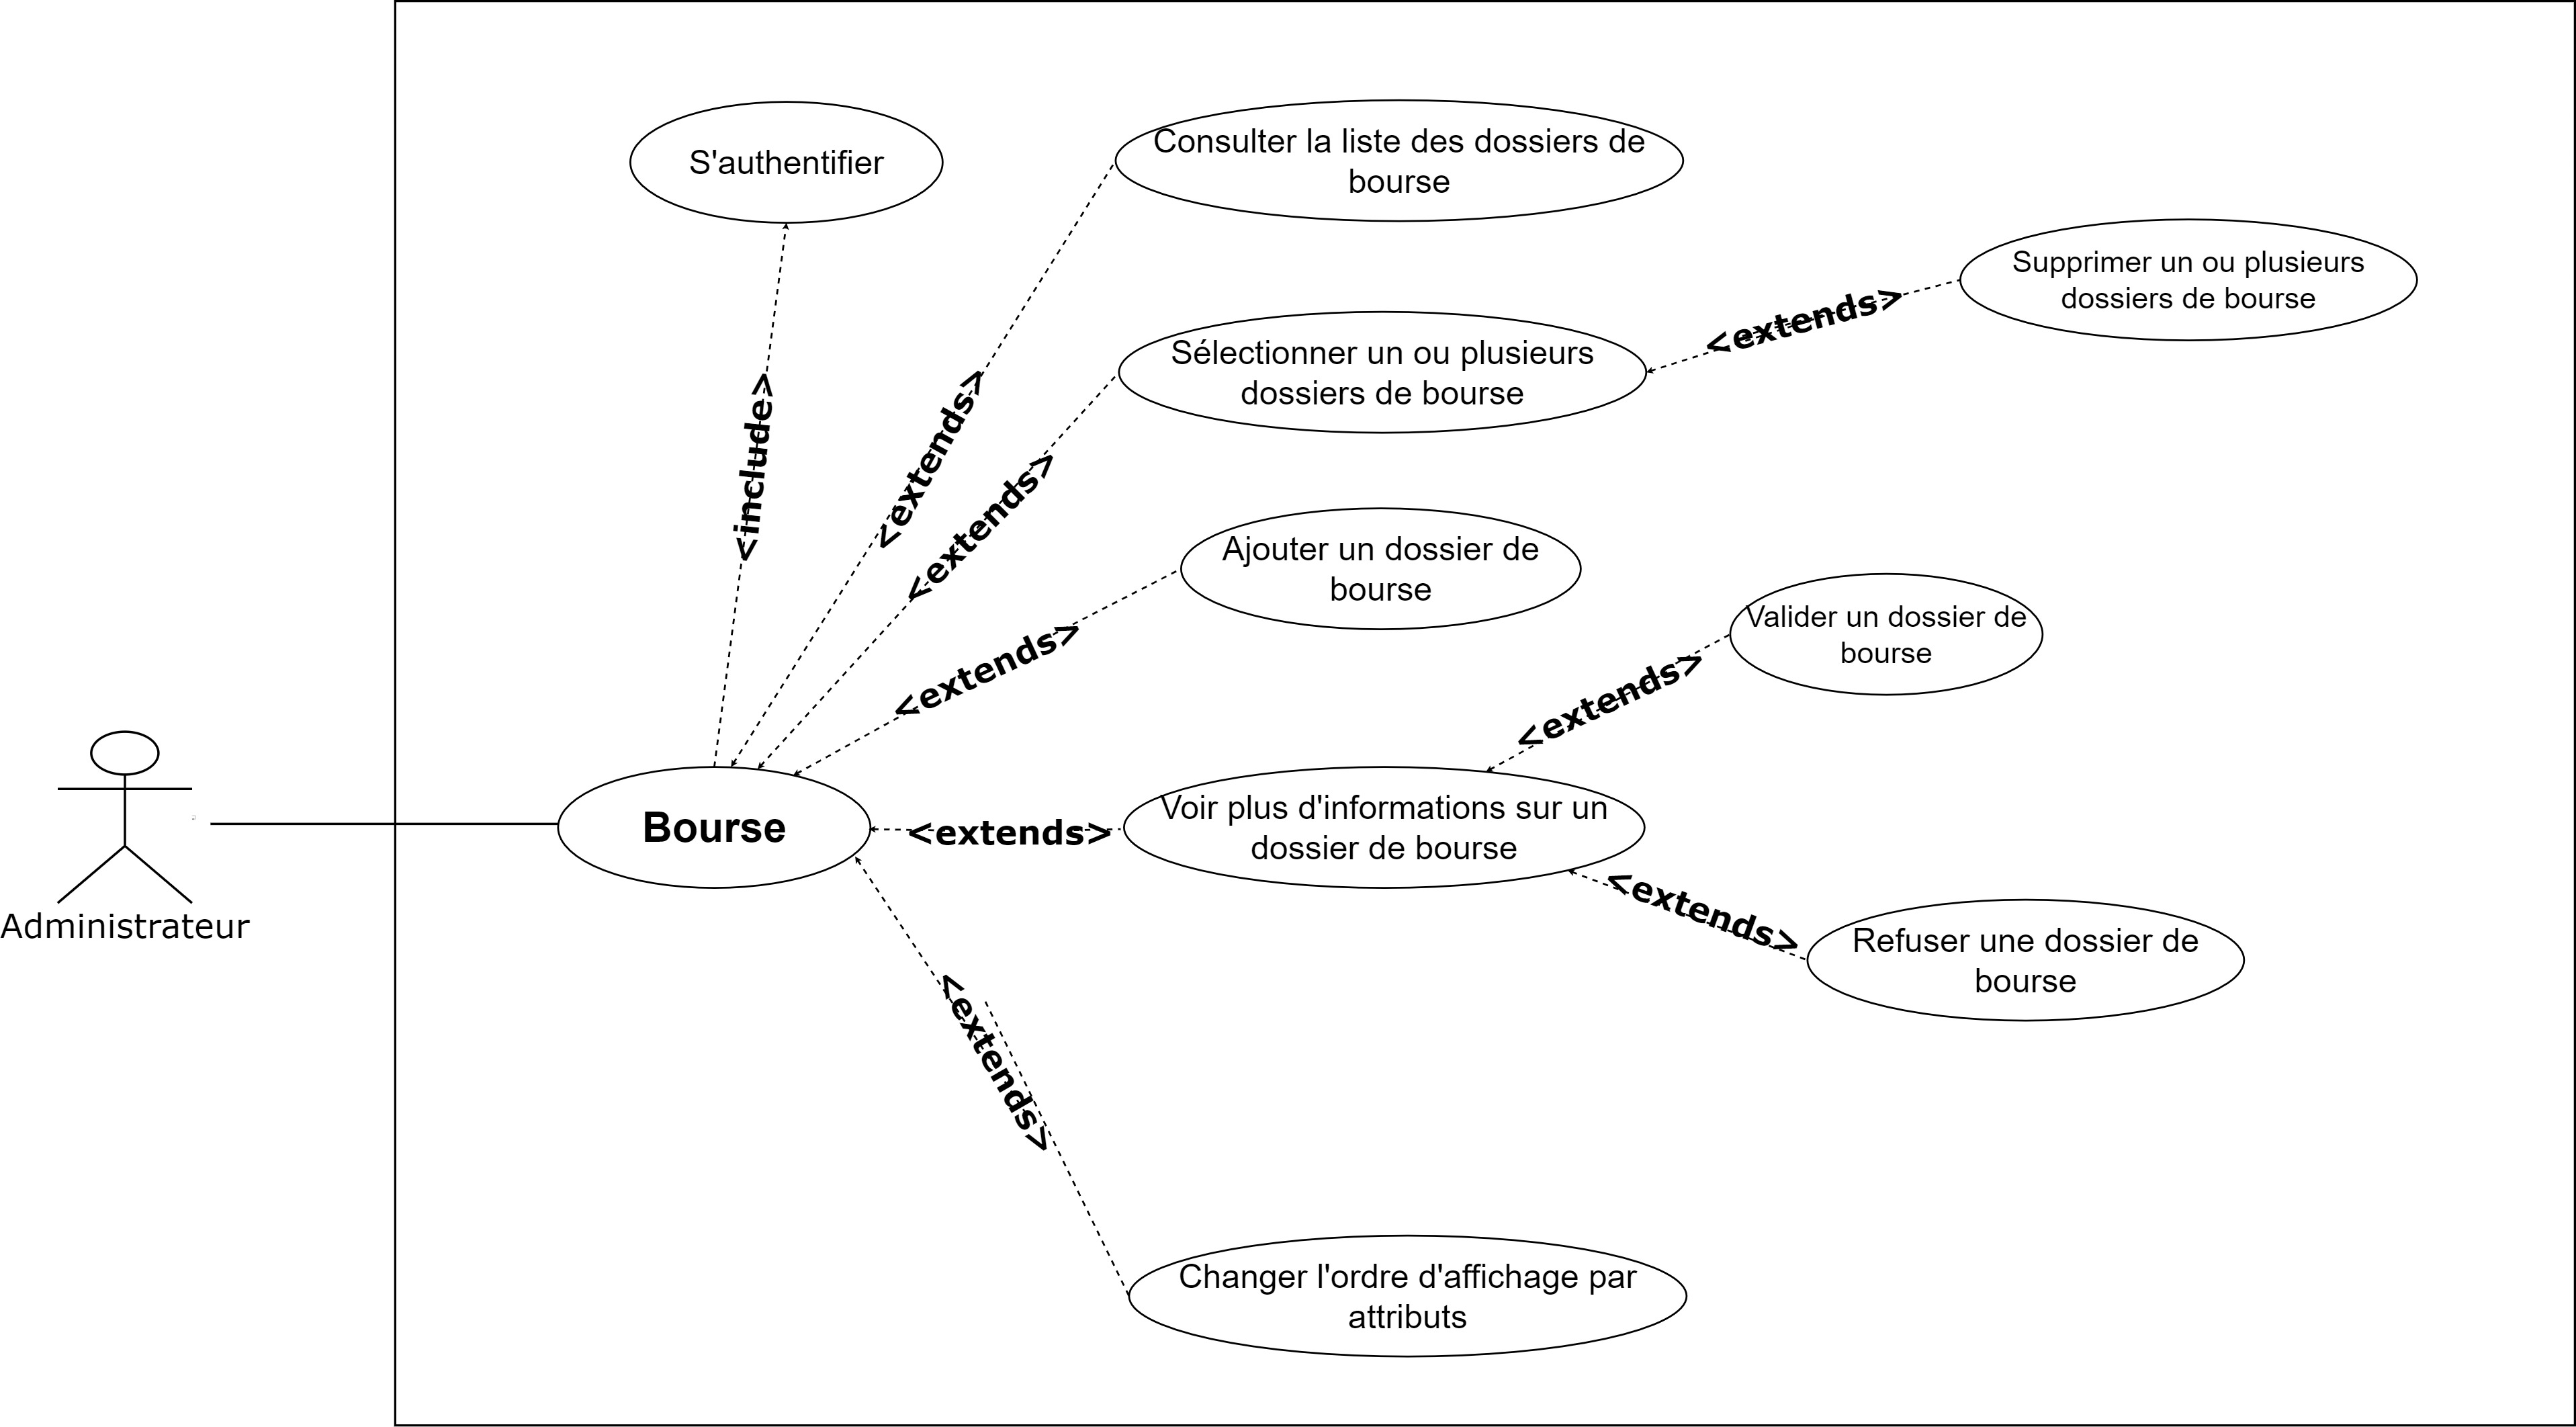
\includegraphics[scale=0.1]{ACR/Diagrammes/Bourse.jpg}
    \caption{Cas d'utilisation 'Bourses'}
\end{figure}

\subsubsection*{Cas d'utilisation 'Campus \& Résidences'}
\begin{figure}[H]
    \centering
    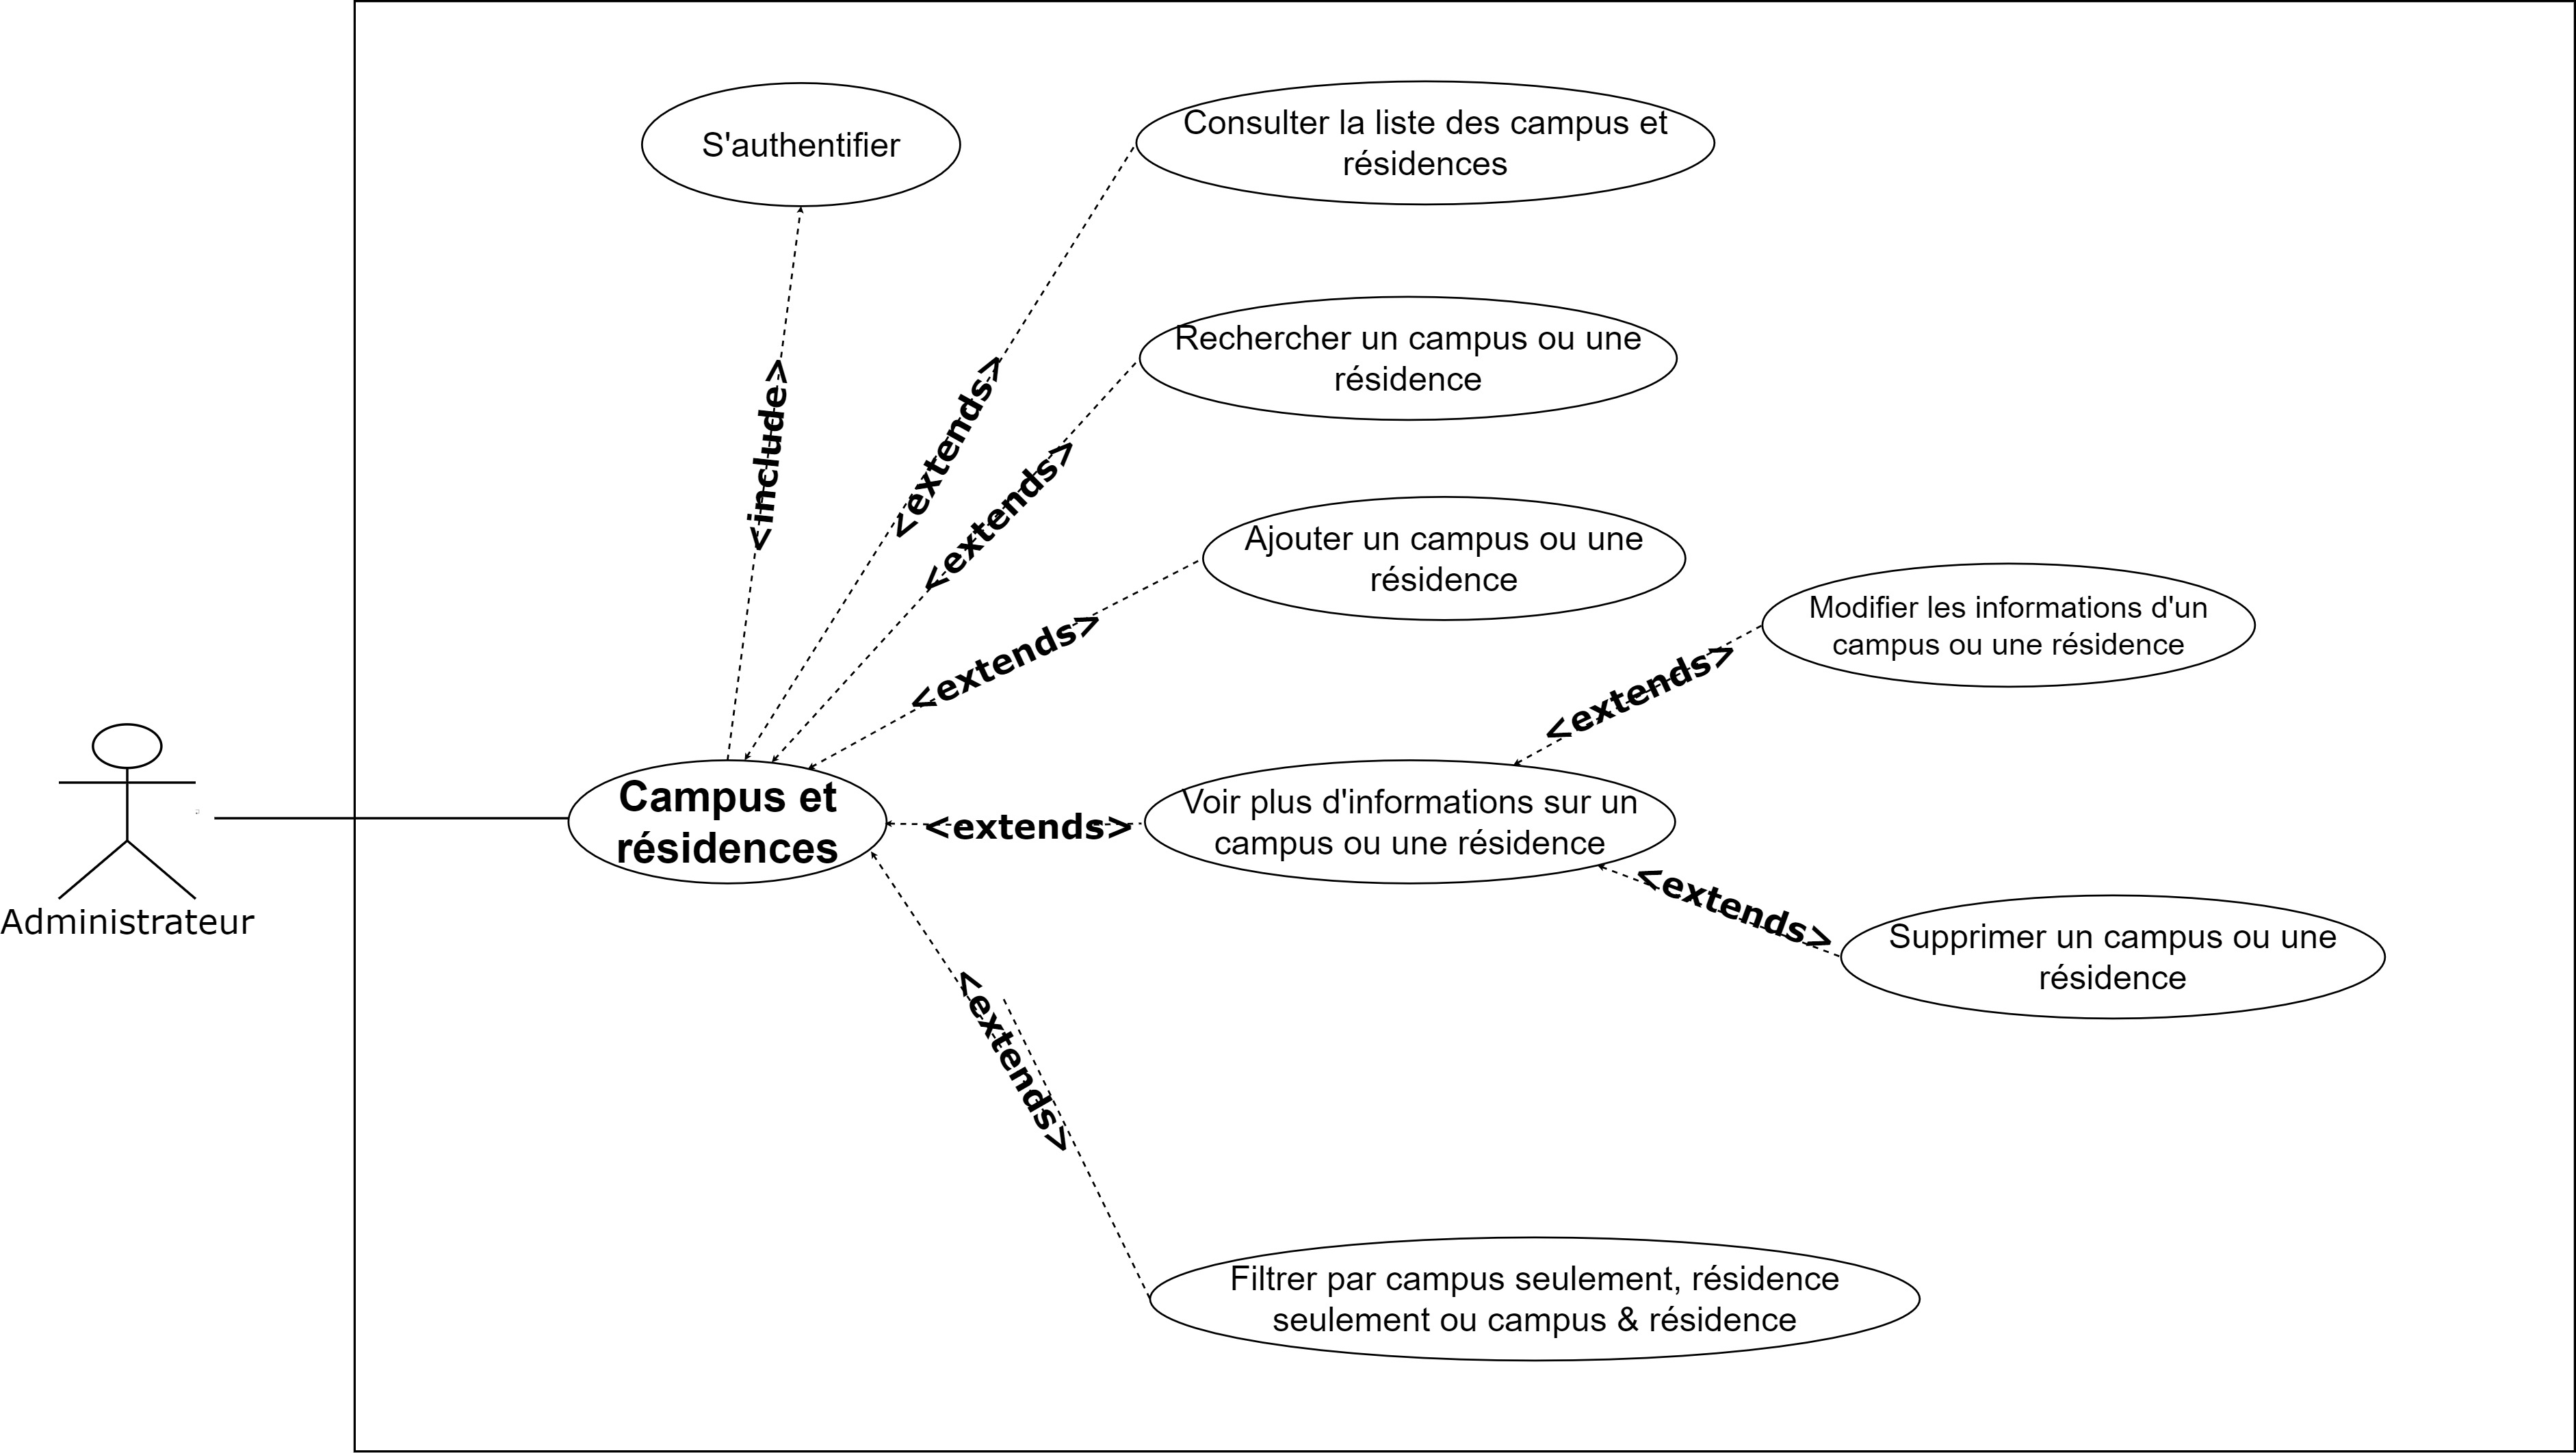
\includegraphics[scale=0.1]{ACR/Diagrammes/Campus-Residences.jpg}
    \caption{Cas d'utilisation 'Campus \& Résidences'}
\end{figure}

\subsubsection*{Cas d'utilisation 'Hébergement'}
\begin{figure}[H]
    \centering
    \includegraphics[scale=0.1]{ACR/Diagrammes/Hébergement.jpg}
    \caption{Cas d'utilisation 'Hébergement'}
\end{figure}

\subsubsection*{Cas d'utilisation 'Page d'accueil'}
\begin{figure}[H]
    \centering
    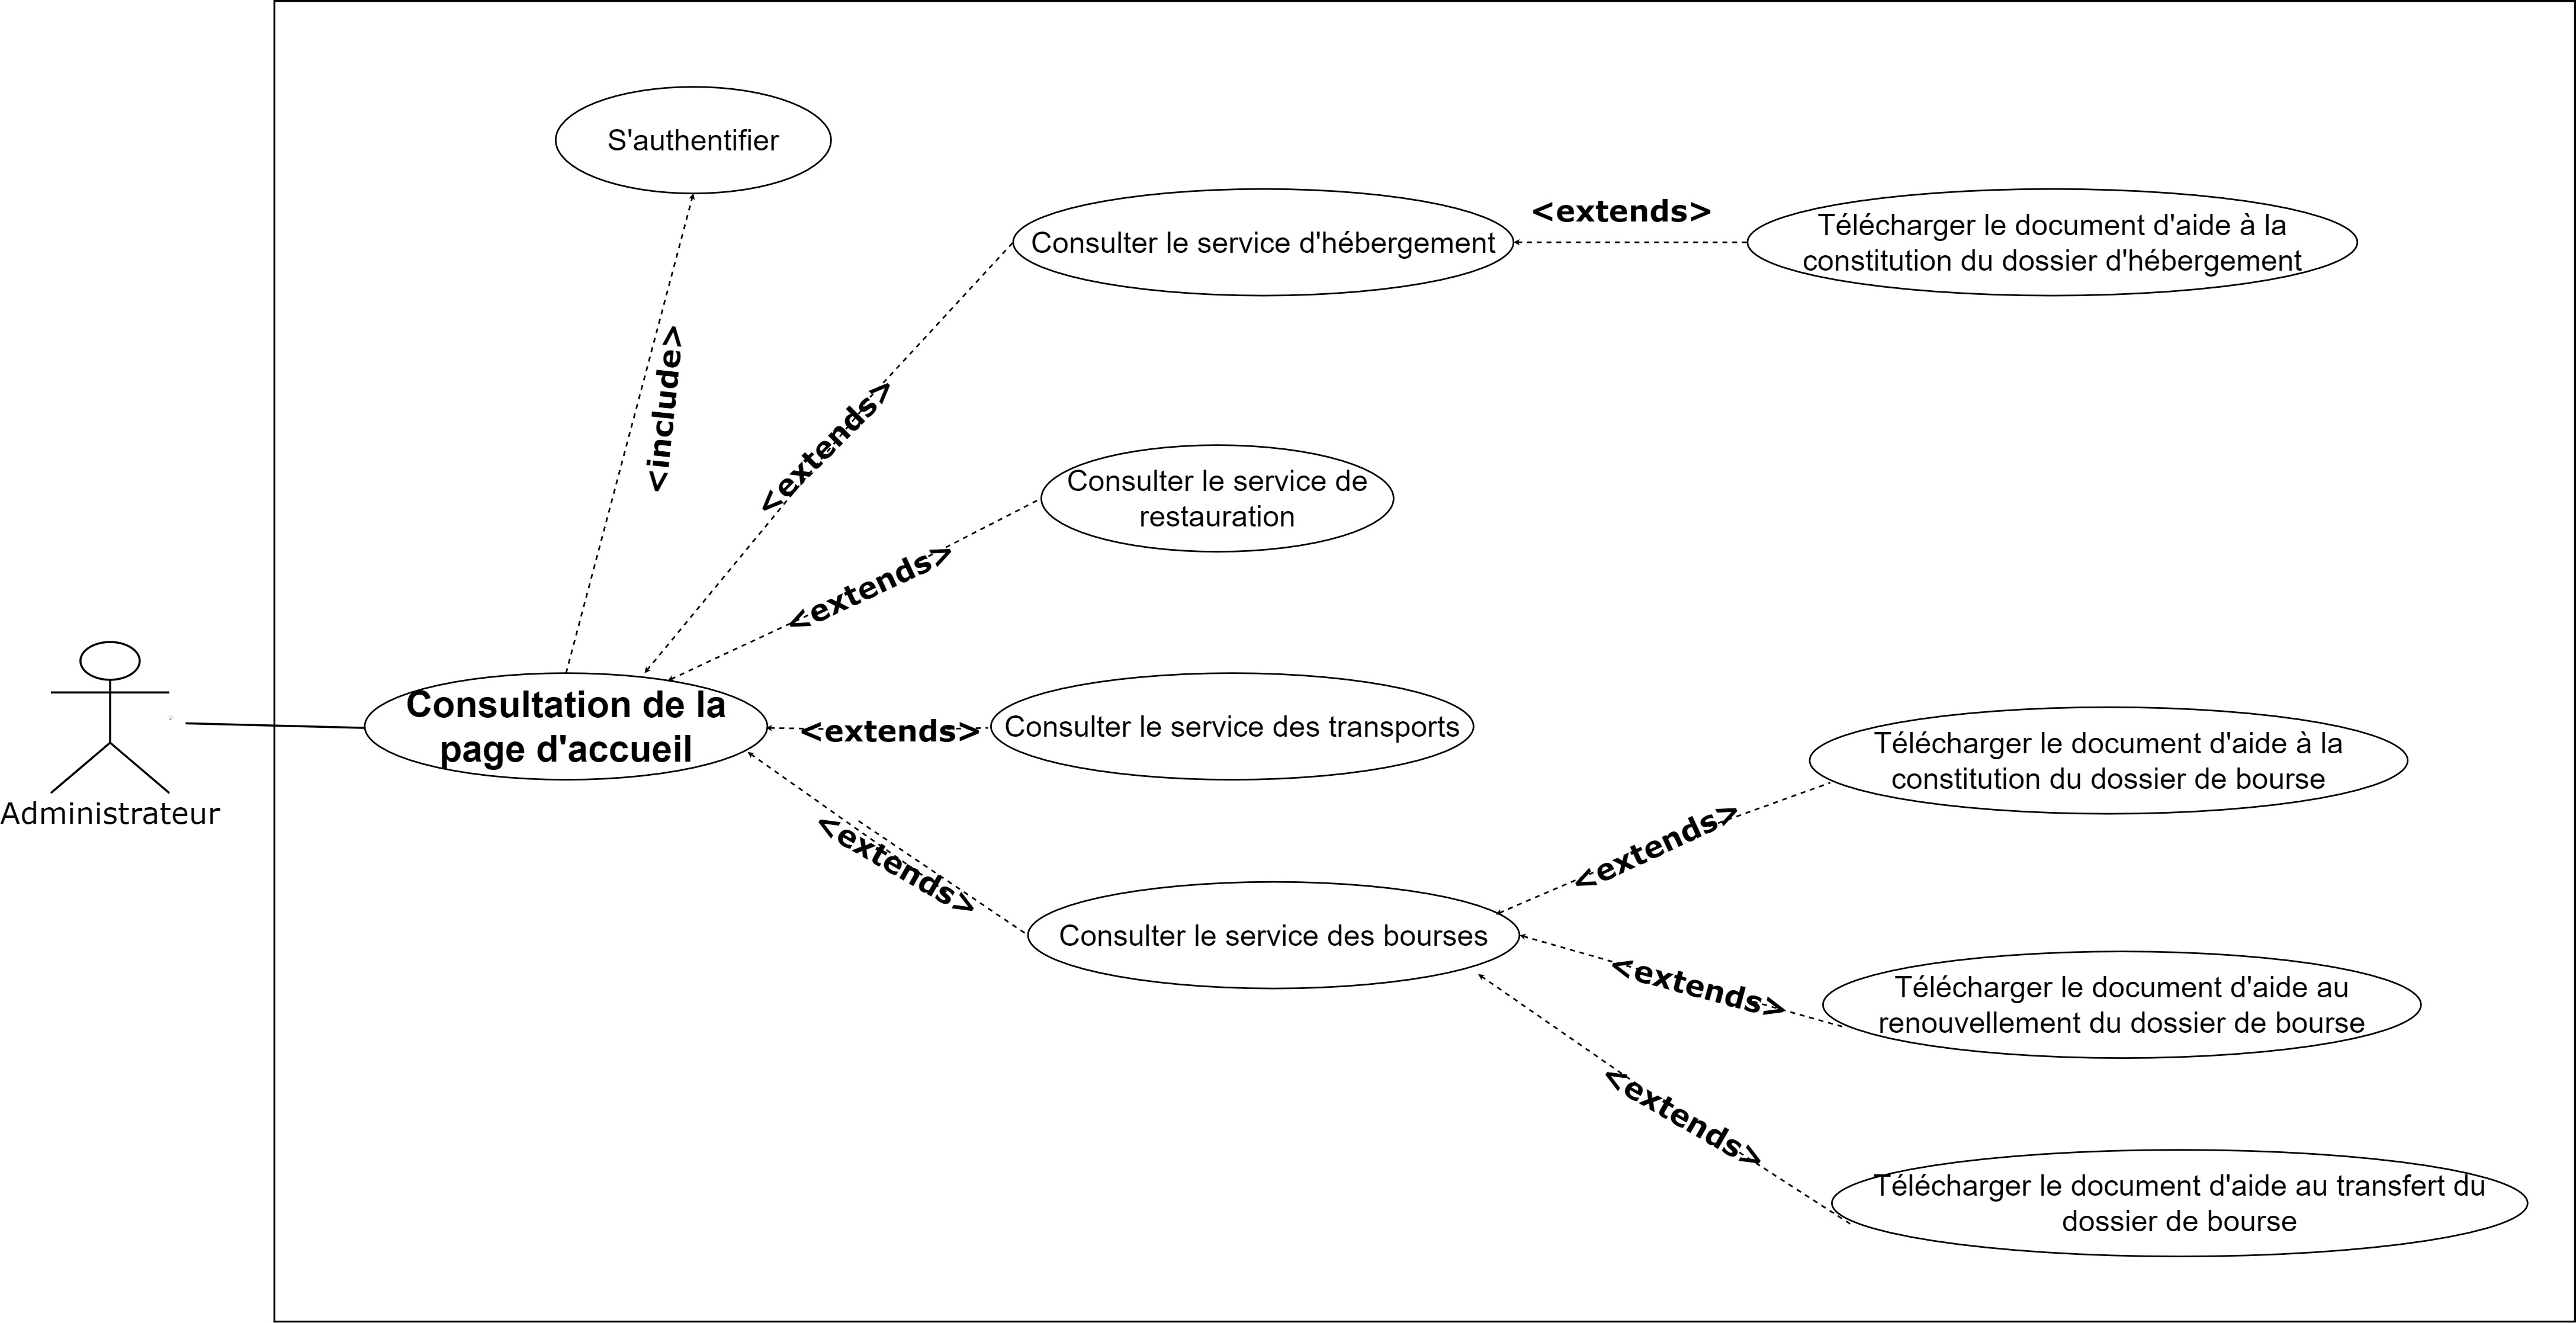
\includegraphics[scale=0.09]{ACR/Diagrammes/accueil.jpg}
    \caption{Cas d'utilisation 'Page d'accueil'}
\end{figure}

\subsubsection*{Cas d'utilisation 'Restauration - Calendrier'}
\begin{figure}[H]
    \centering
    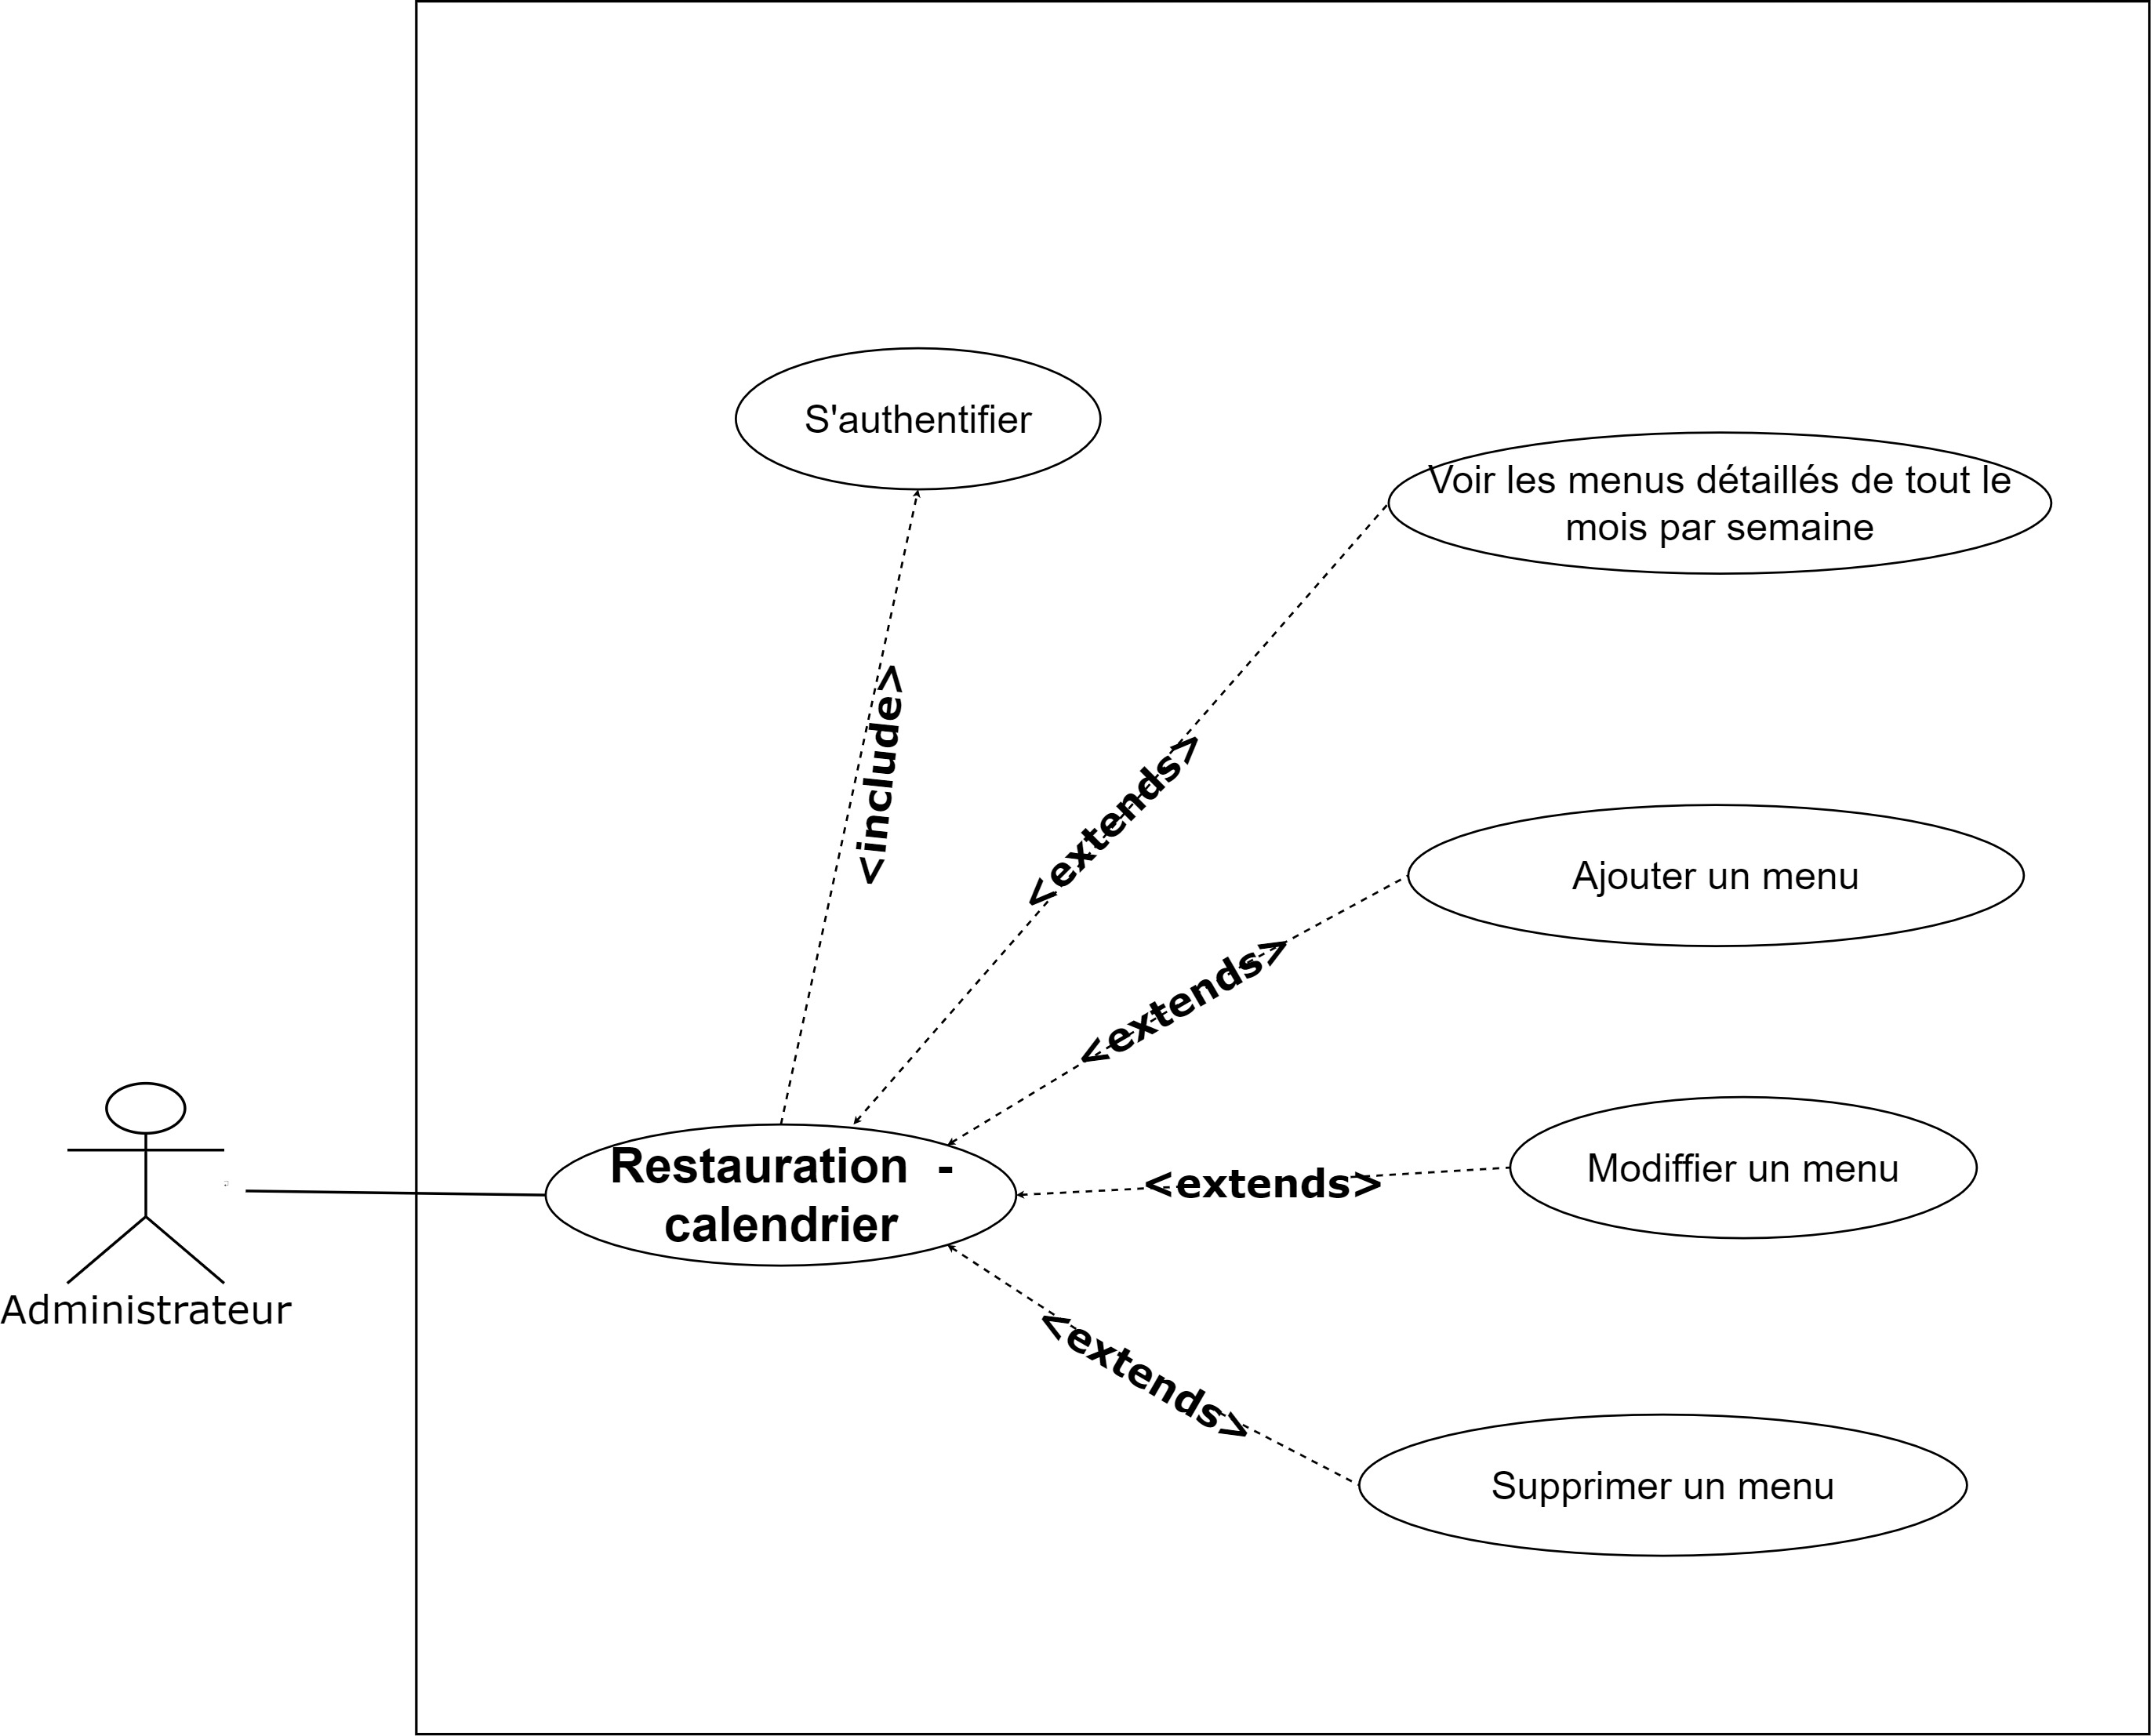
\includegraphics[scale=0.1]{ACR/Diagrammes/Restauration - calendrier.jpg}
    \caption{Cas d'utilisation 'Restauration - Calendrier'}
\end{figure}

\subsubsection*{Cas d'utilisation 'Restauration - Ingrédients'}
\begin{figure}[H]
    \centering
    \includegraphics[scale=0.1]{ACR/Diagrammes/Restauration - ingrédients.jpg}
    \caption{Cas d'utilisation 'Restauration - Ingrédients'}
\end{figure}

\subsubsection*{Cas d'utilisation 'Restauration - Plats \& Desserts'}
\begin{figure}[H]
    \centering
    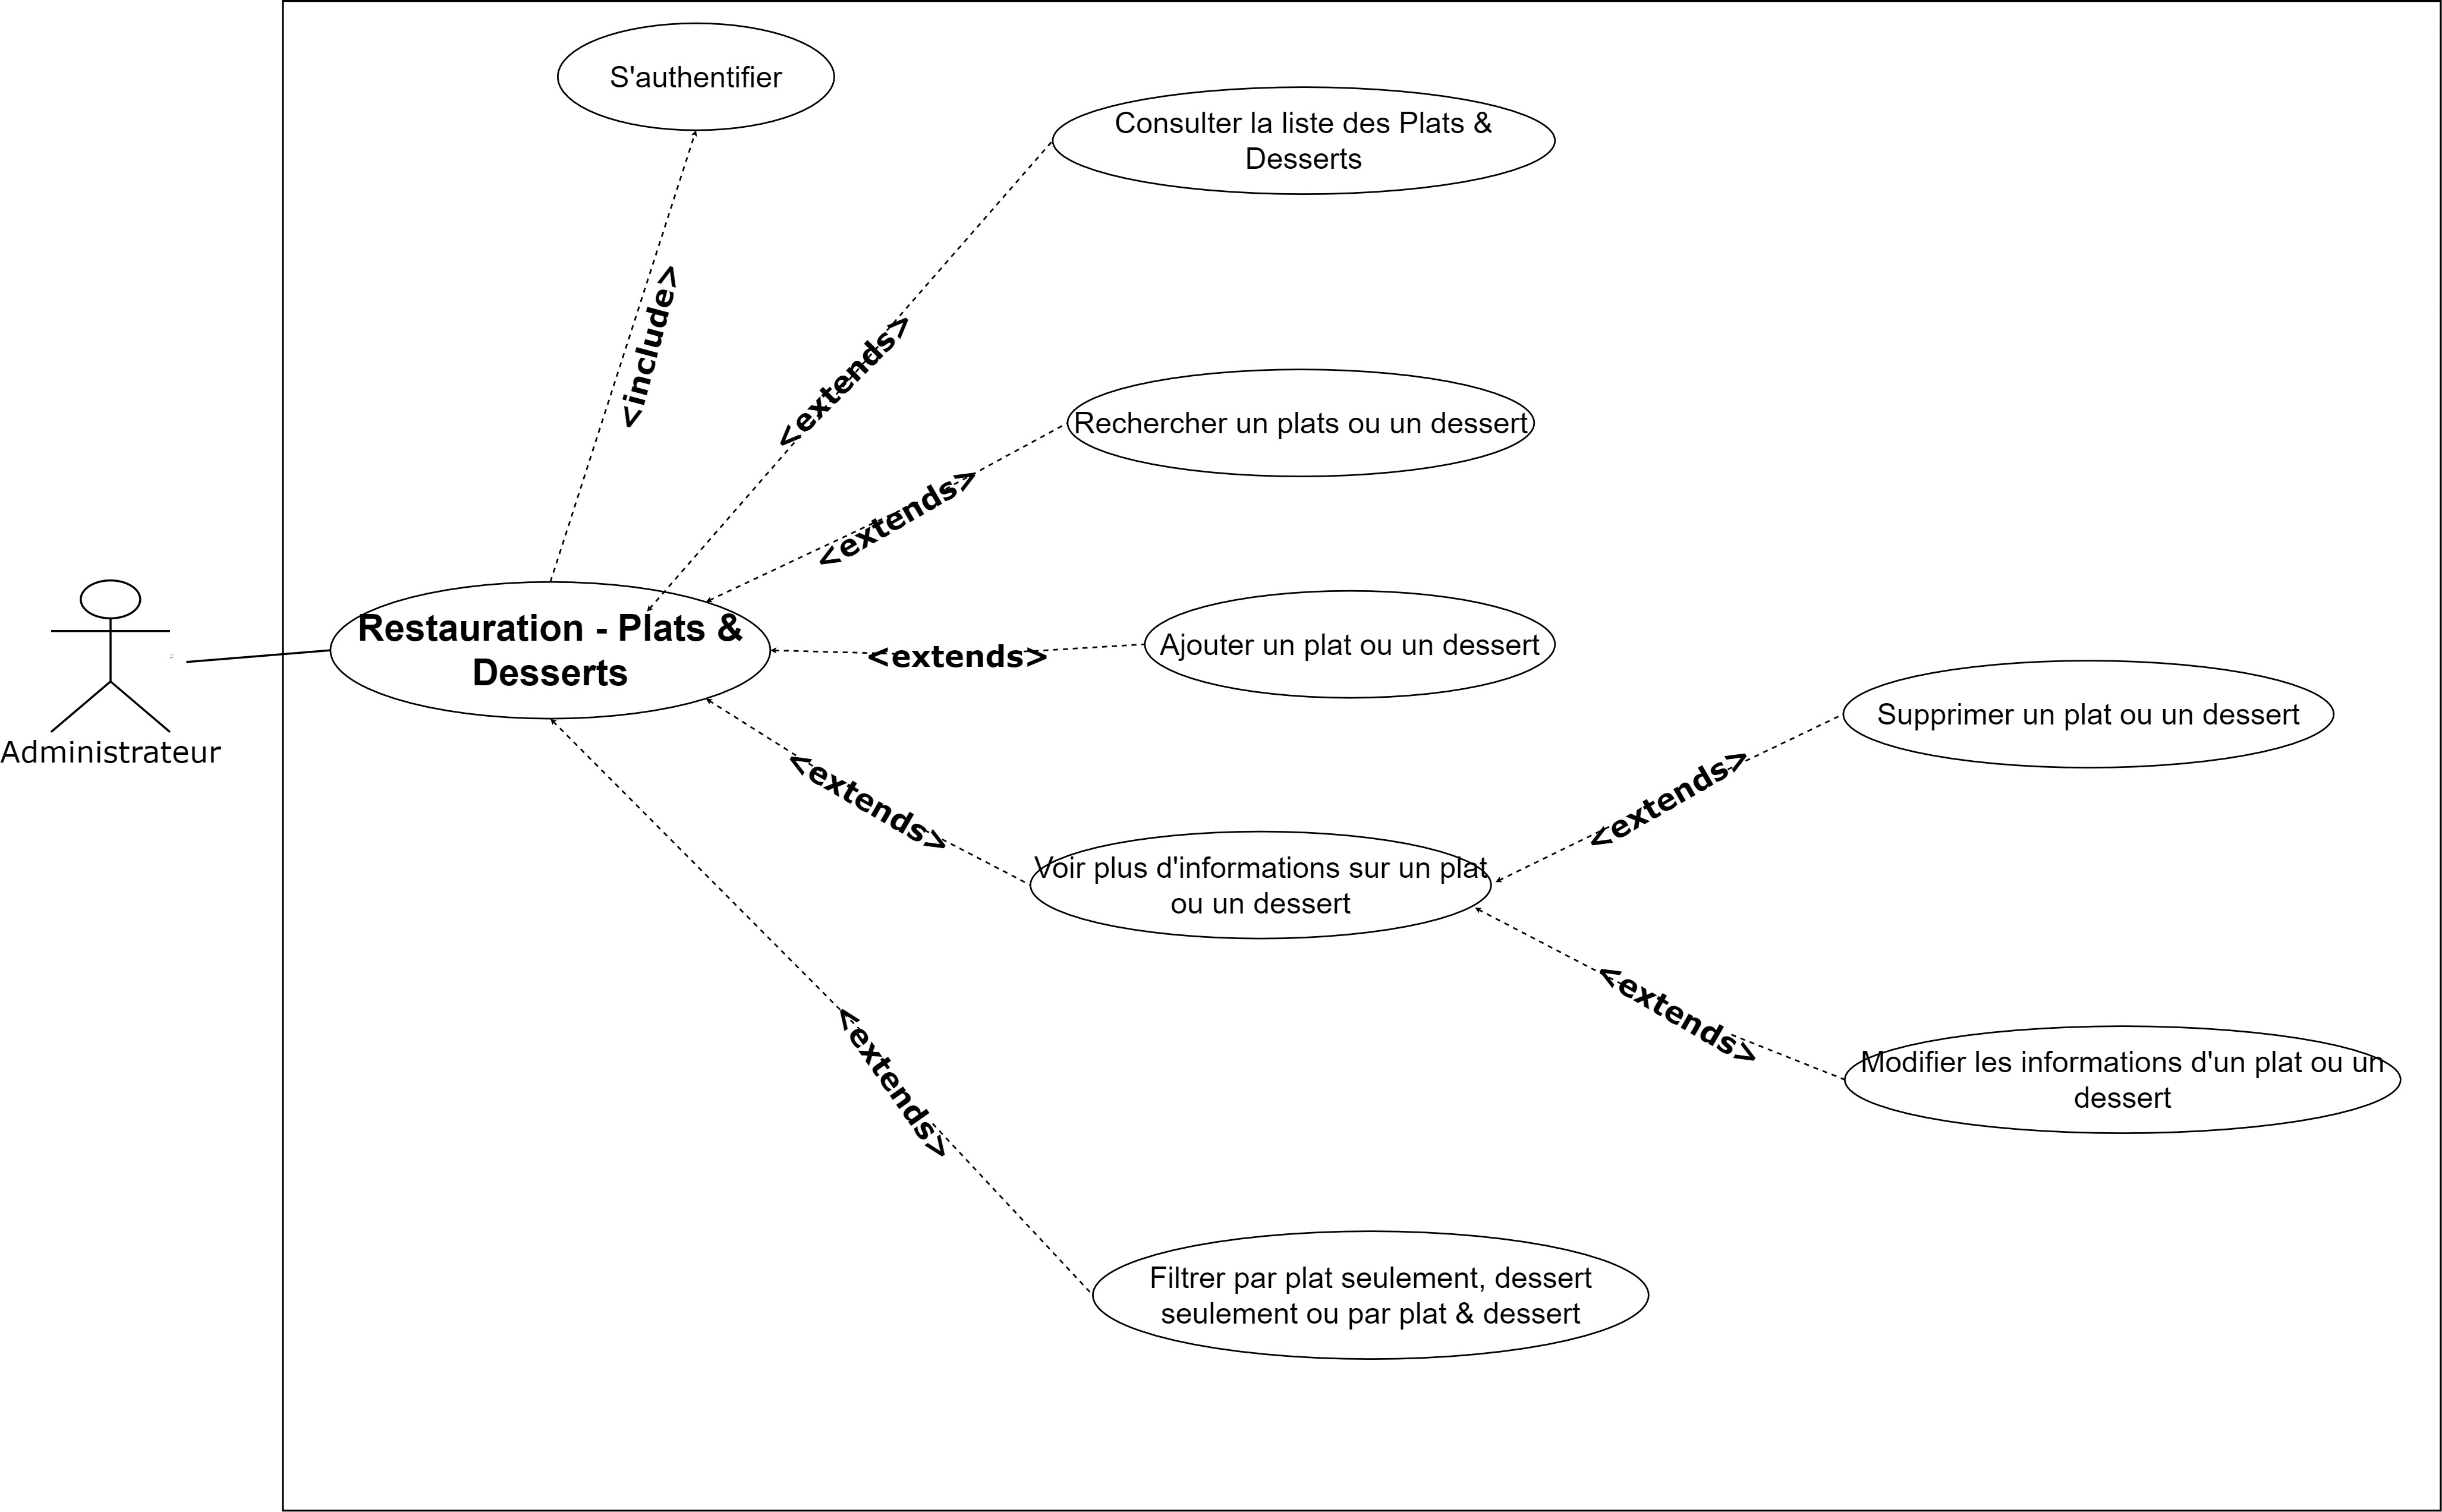
\includegraphics[scale=0.1]{ACR/Diagrammes/Restauration - Plats&Desserts.jpg}
    \caption{Cas d'utilisation 'Restauration - Plats \& Desserts'}
\end{figure}

\subsubsection*{Cas d'utilisation 'Restauration - Restaurants'}
\begin{figure}[H]
    \centering
    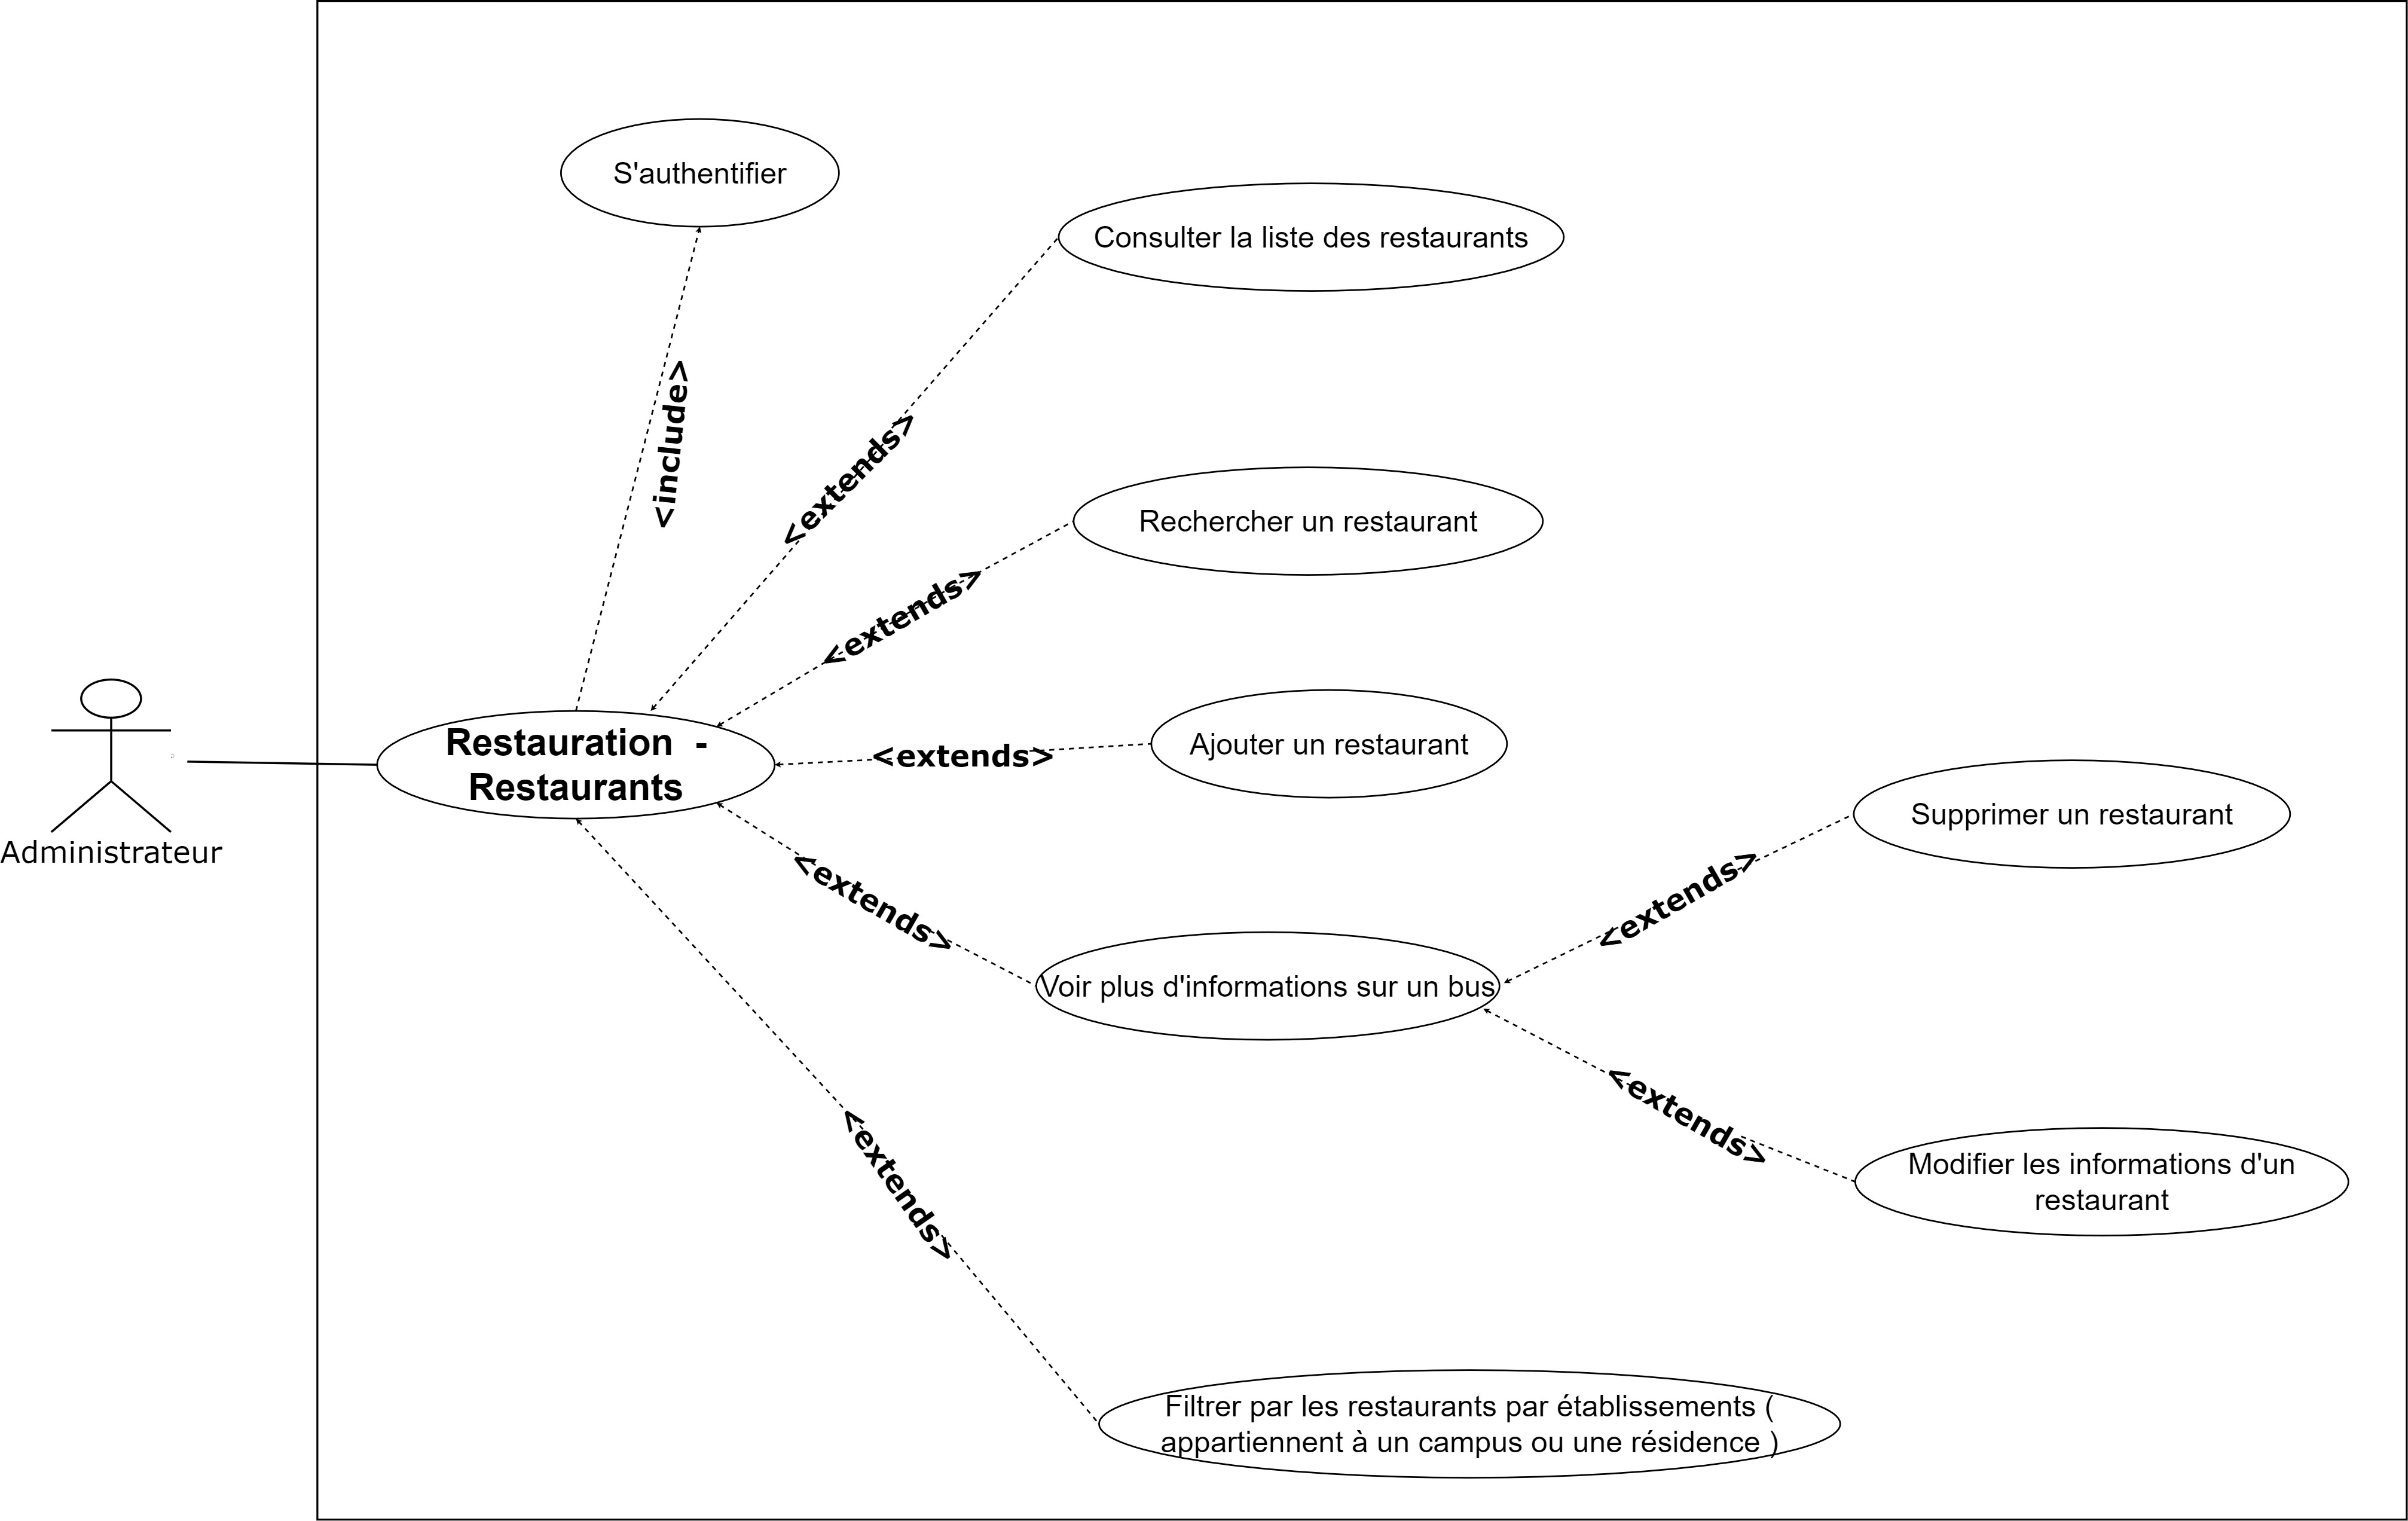
\includegraphics[scale=0.1]{ACR/Diagrammes/Restauration - restaurants.jpg}
    \caption{Cas d'utilisation 'Restauration - Restaurants'}
\end{figure}

\subsubsection*{Cas d'utilisation 'Transports - Bus'}
\begin{figure}[H]
    \centering
    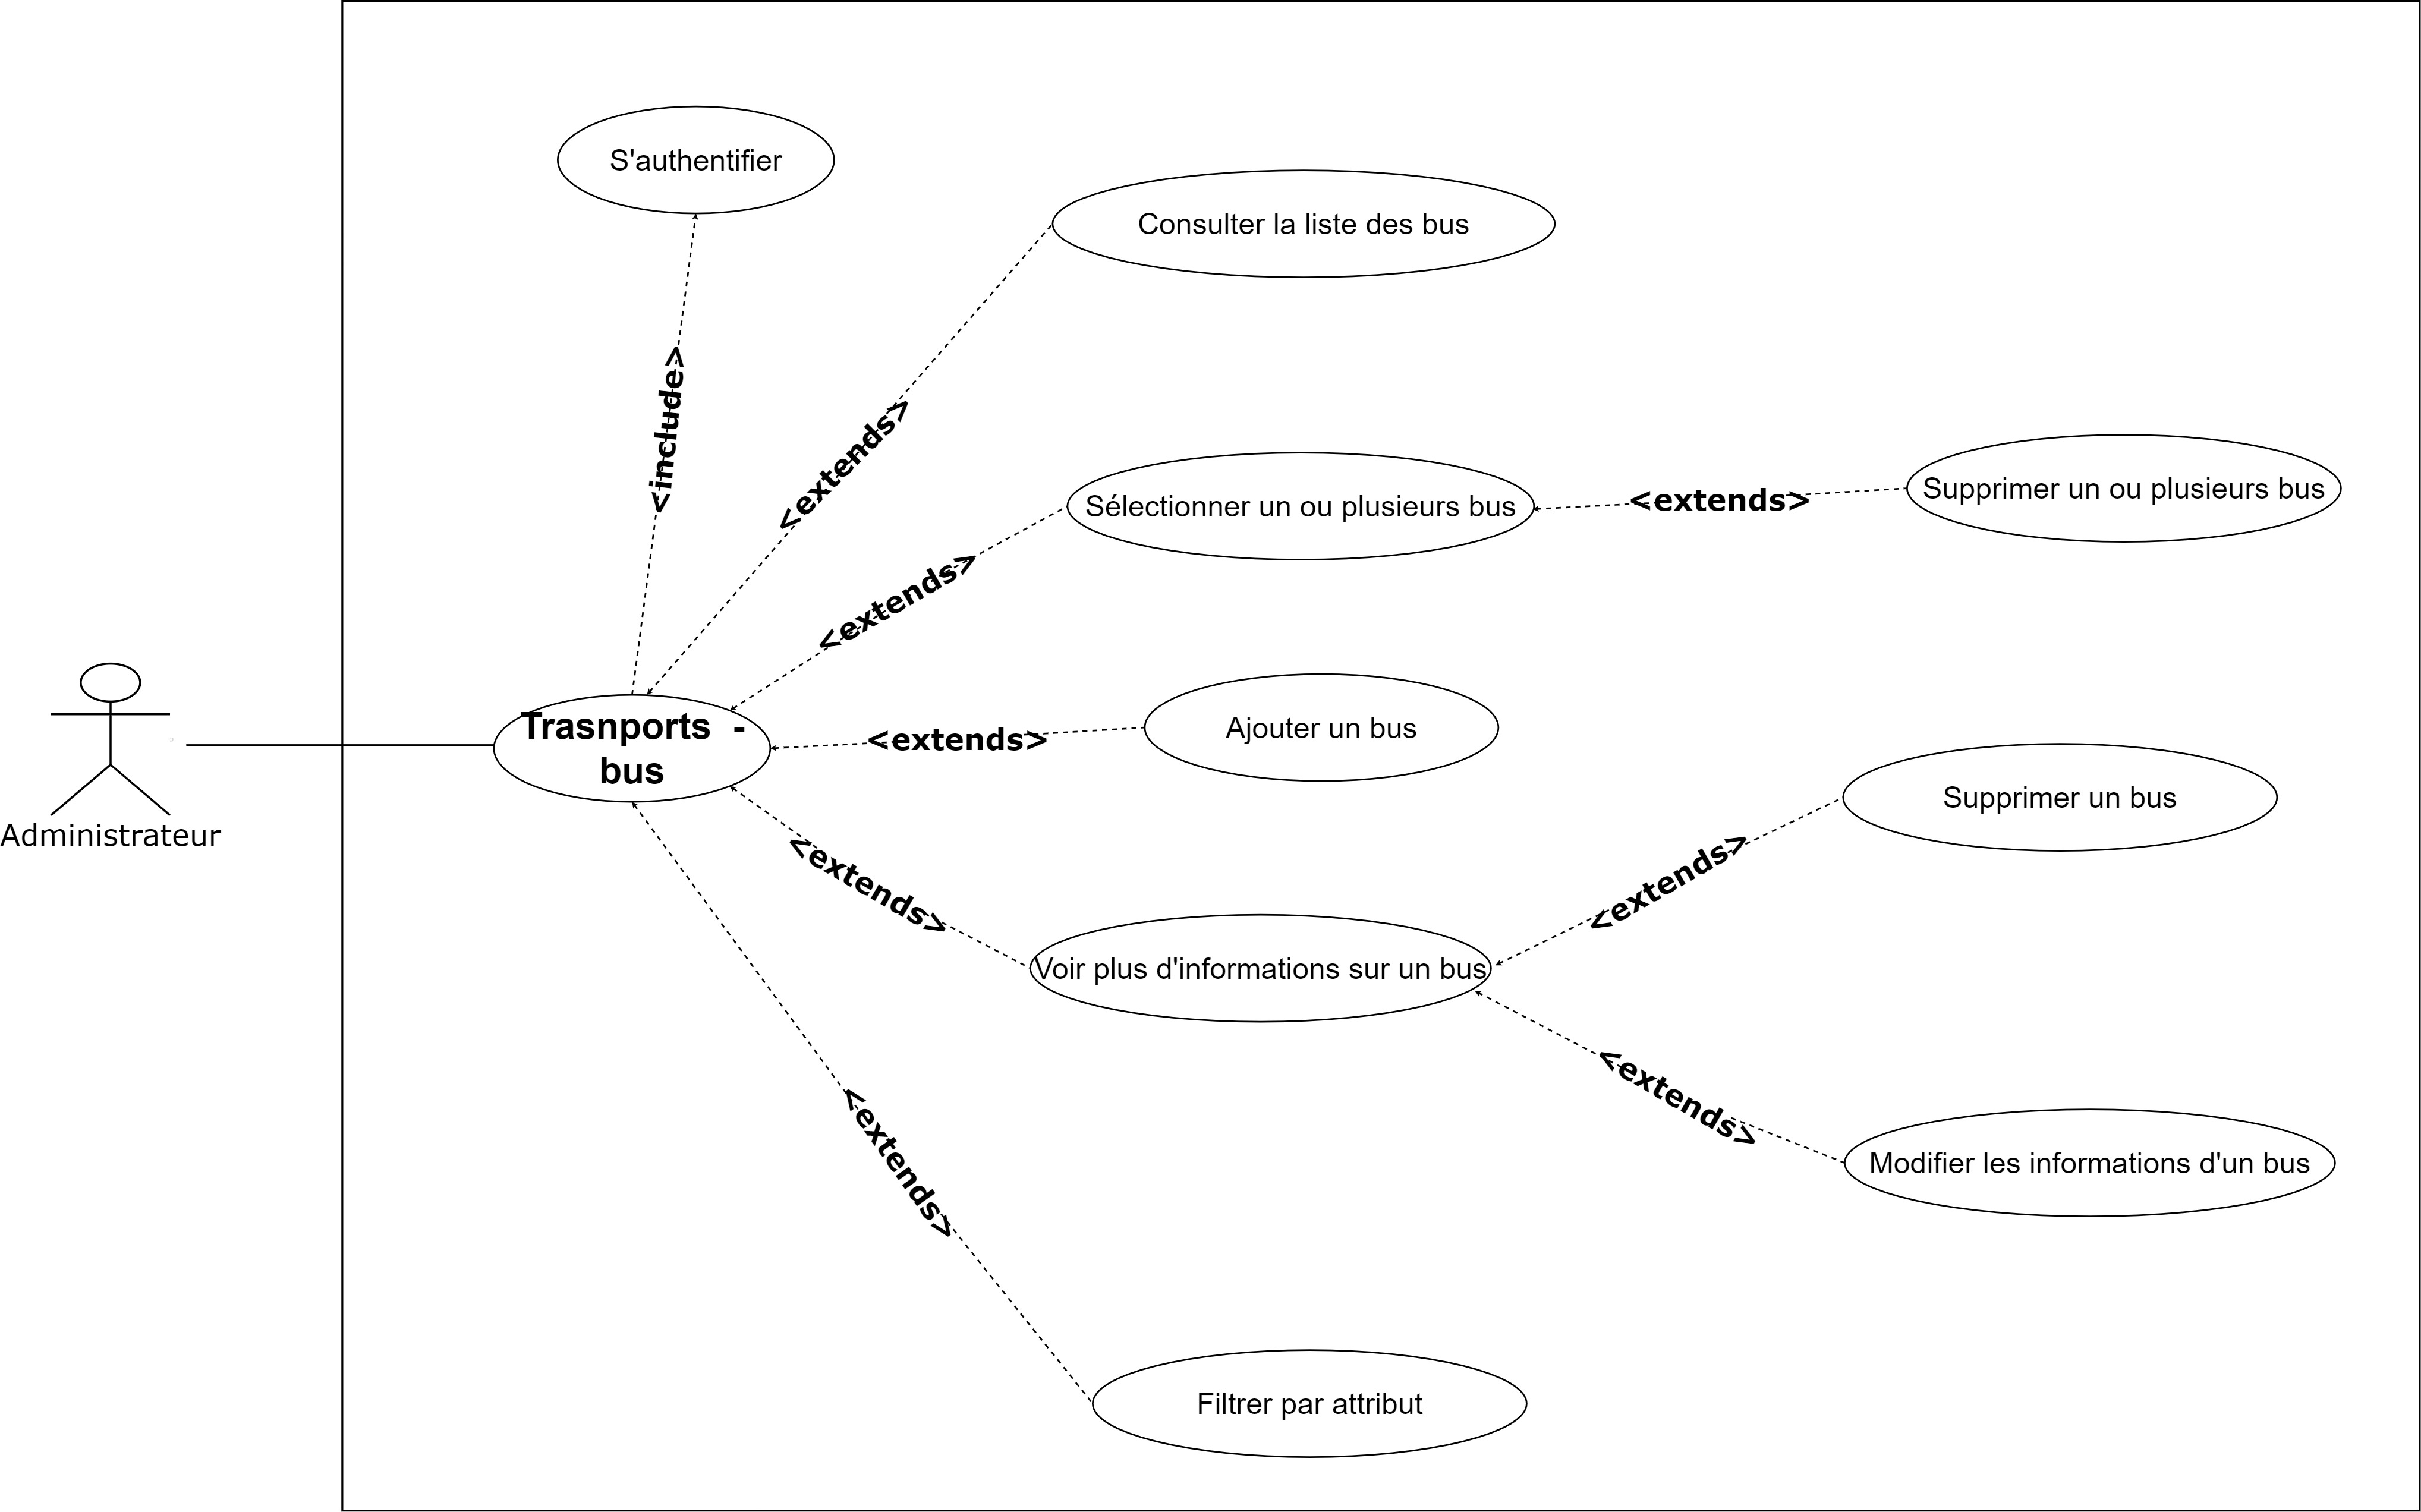
\includegraphics[scale=0.1]{ACR/Diagrammes/Transports - bus.jpg}
    \caption{Cas d'utilisation 'Transports - Bus'}
\end{figure}

\subsubsection*{Cas d'utilisation 'Transports - Calendrier'}
\begin{figure}[H]
    \centering
    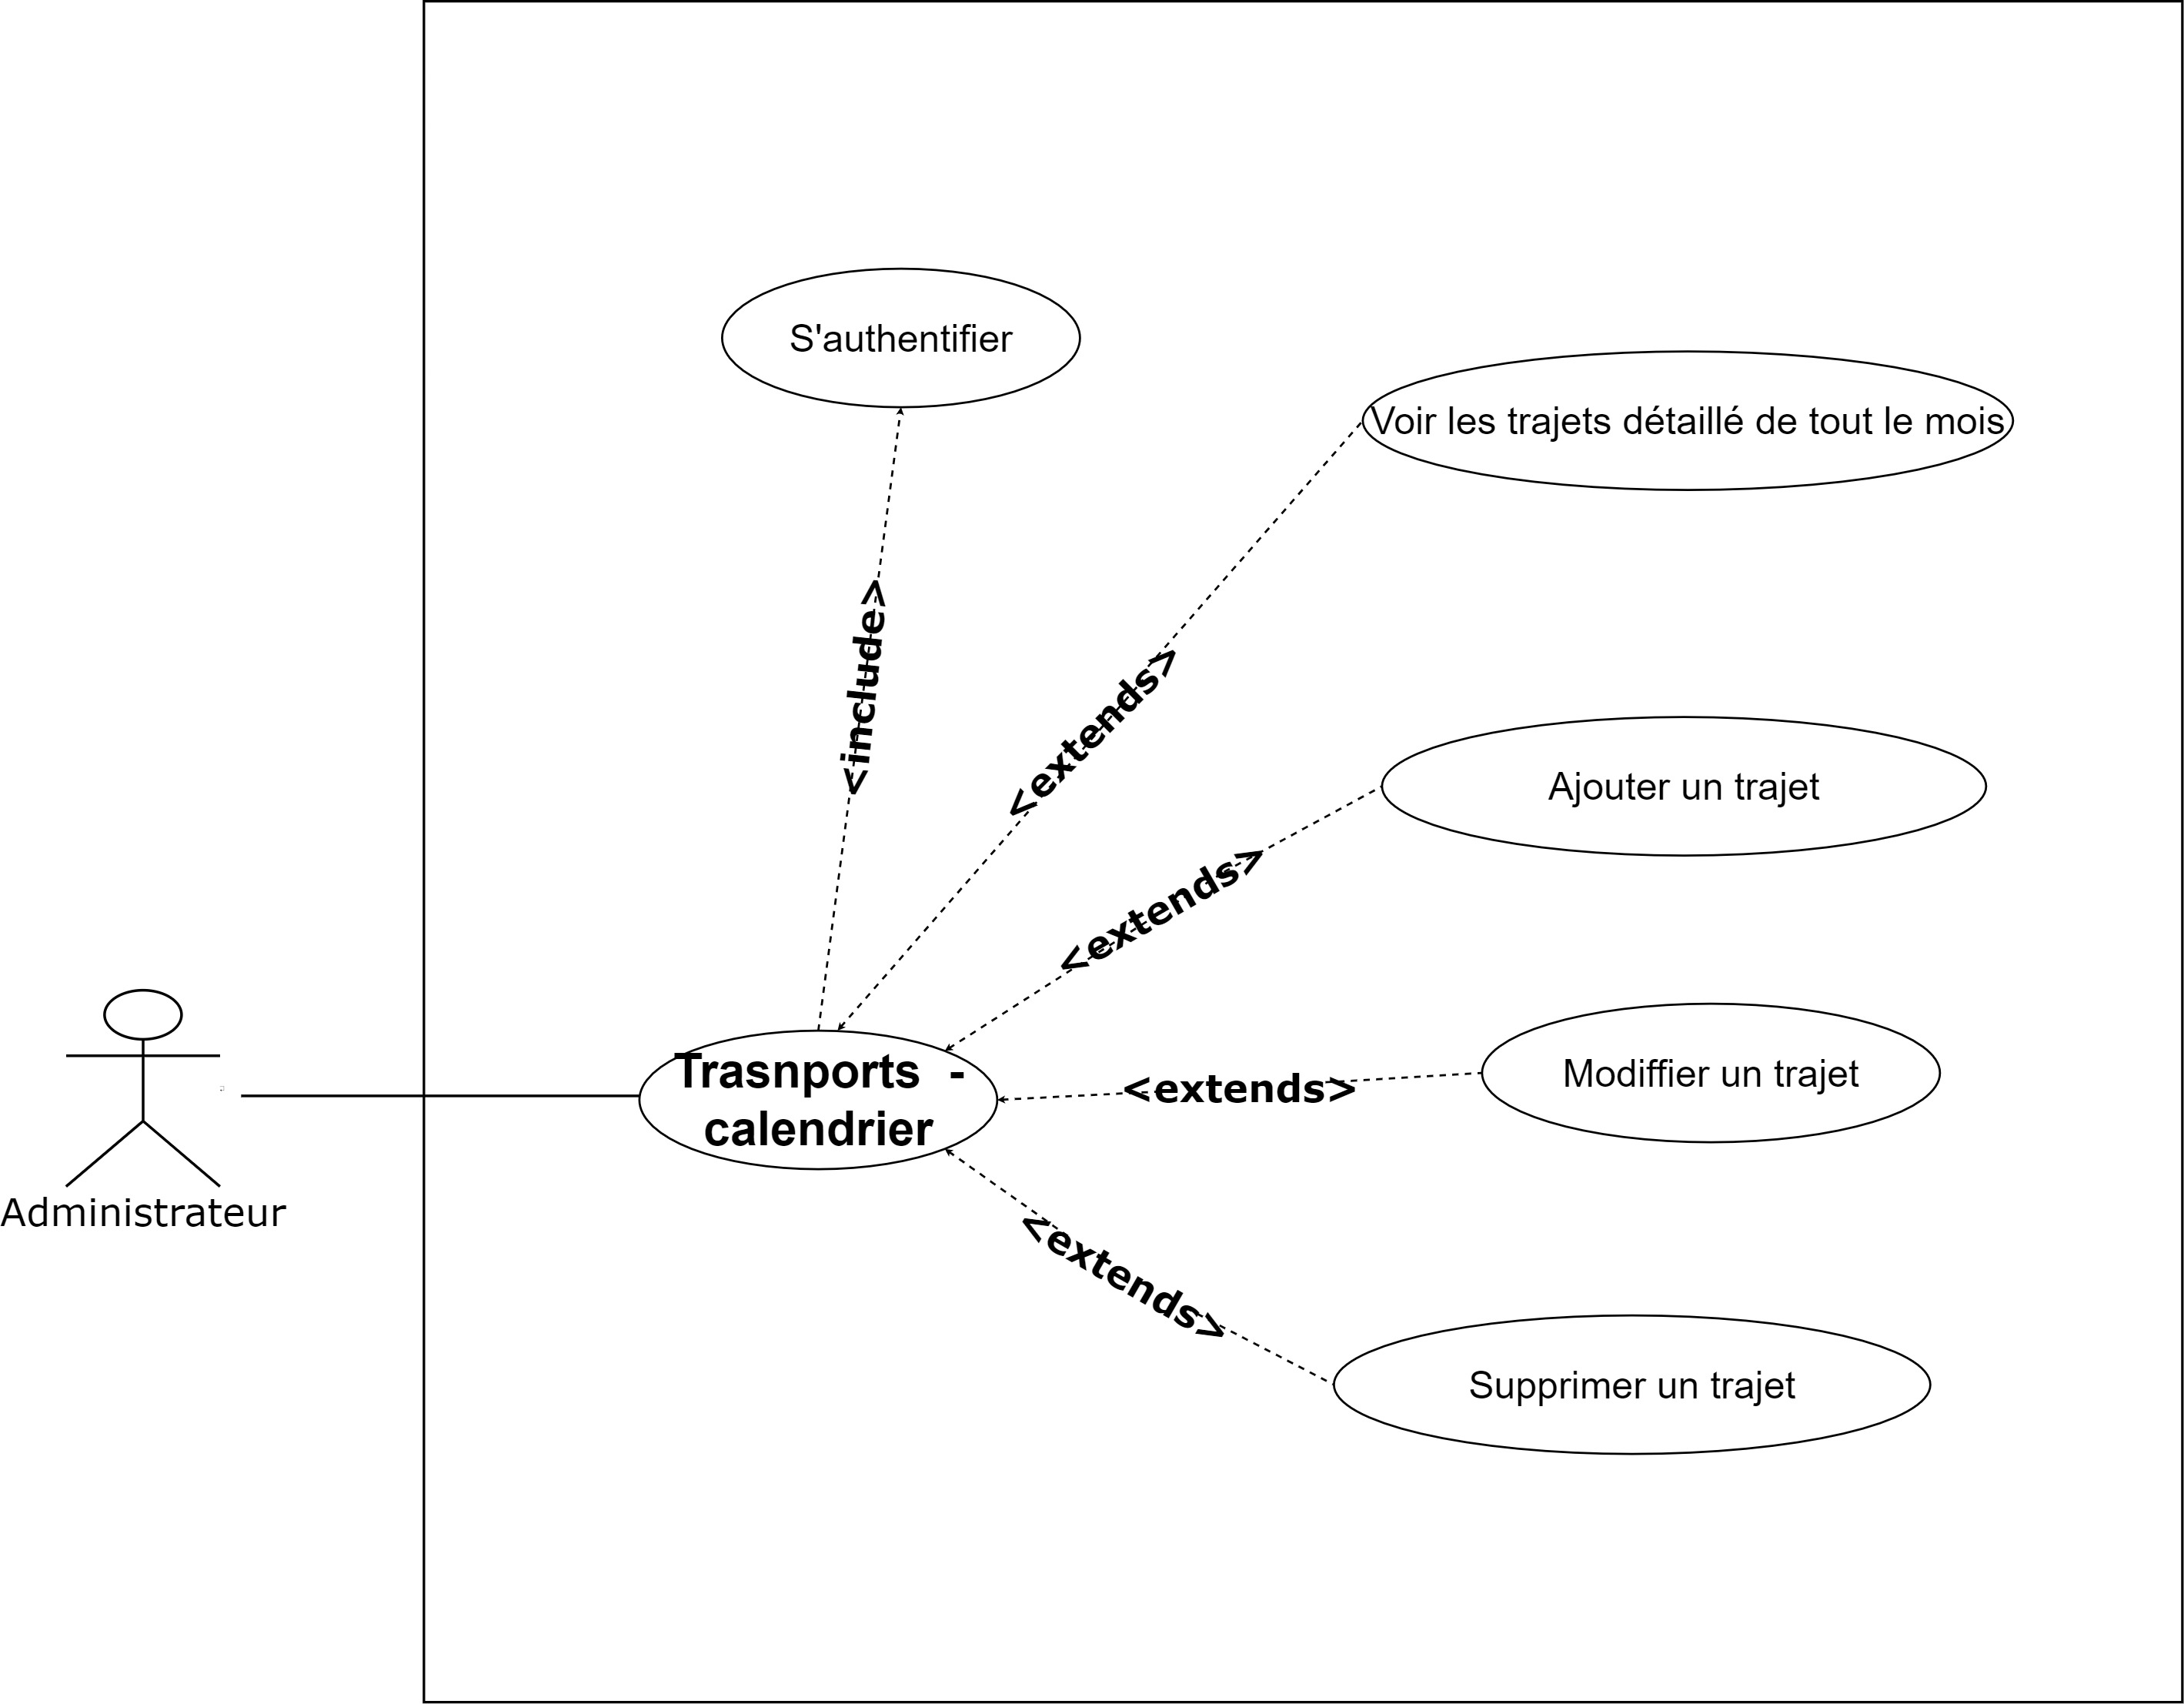
\includegraphics[scale=0.1]{ACR/Diagrammes/Transports - calendrier.jpg}
    \caption{Cas d'utilisation 'Transports - Calendrier'}
\end{figure}

\subsubsection*{Cas d'utilisation 'Utilisateurs'}
\begin{figure}[H]
    \centering
    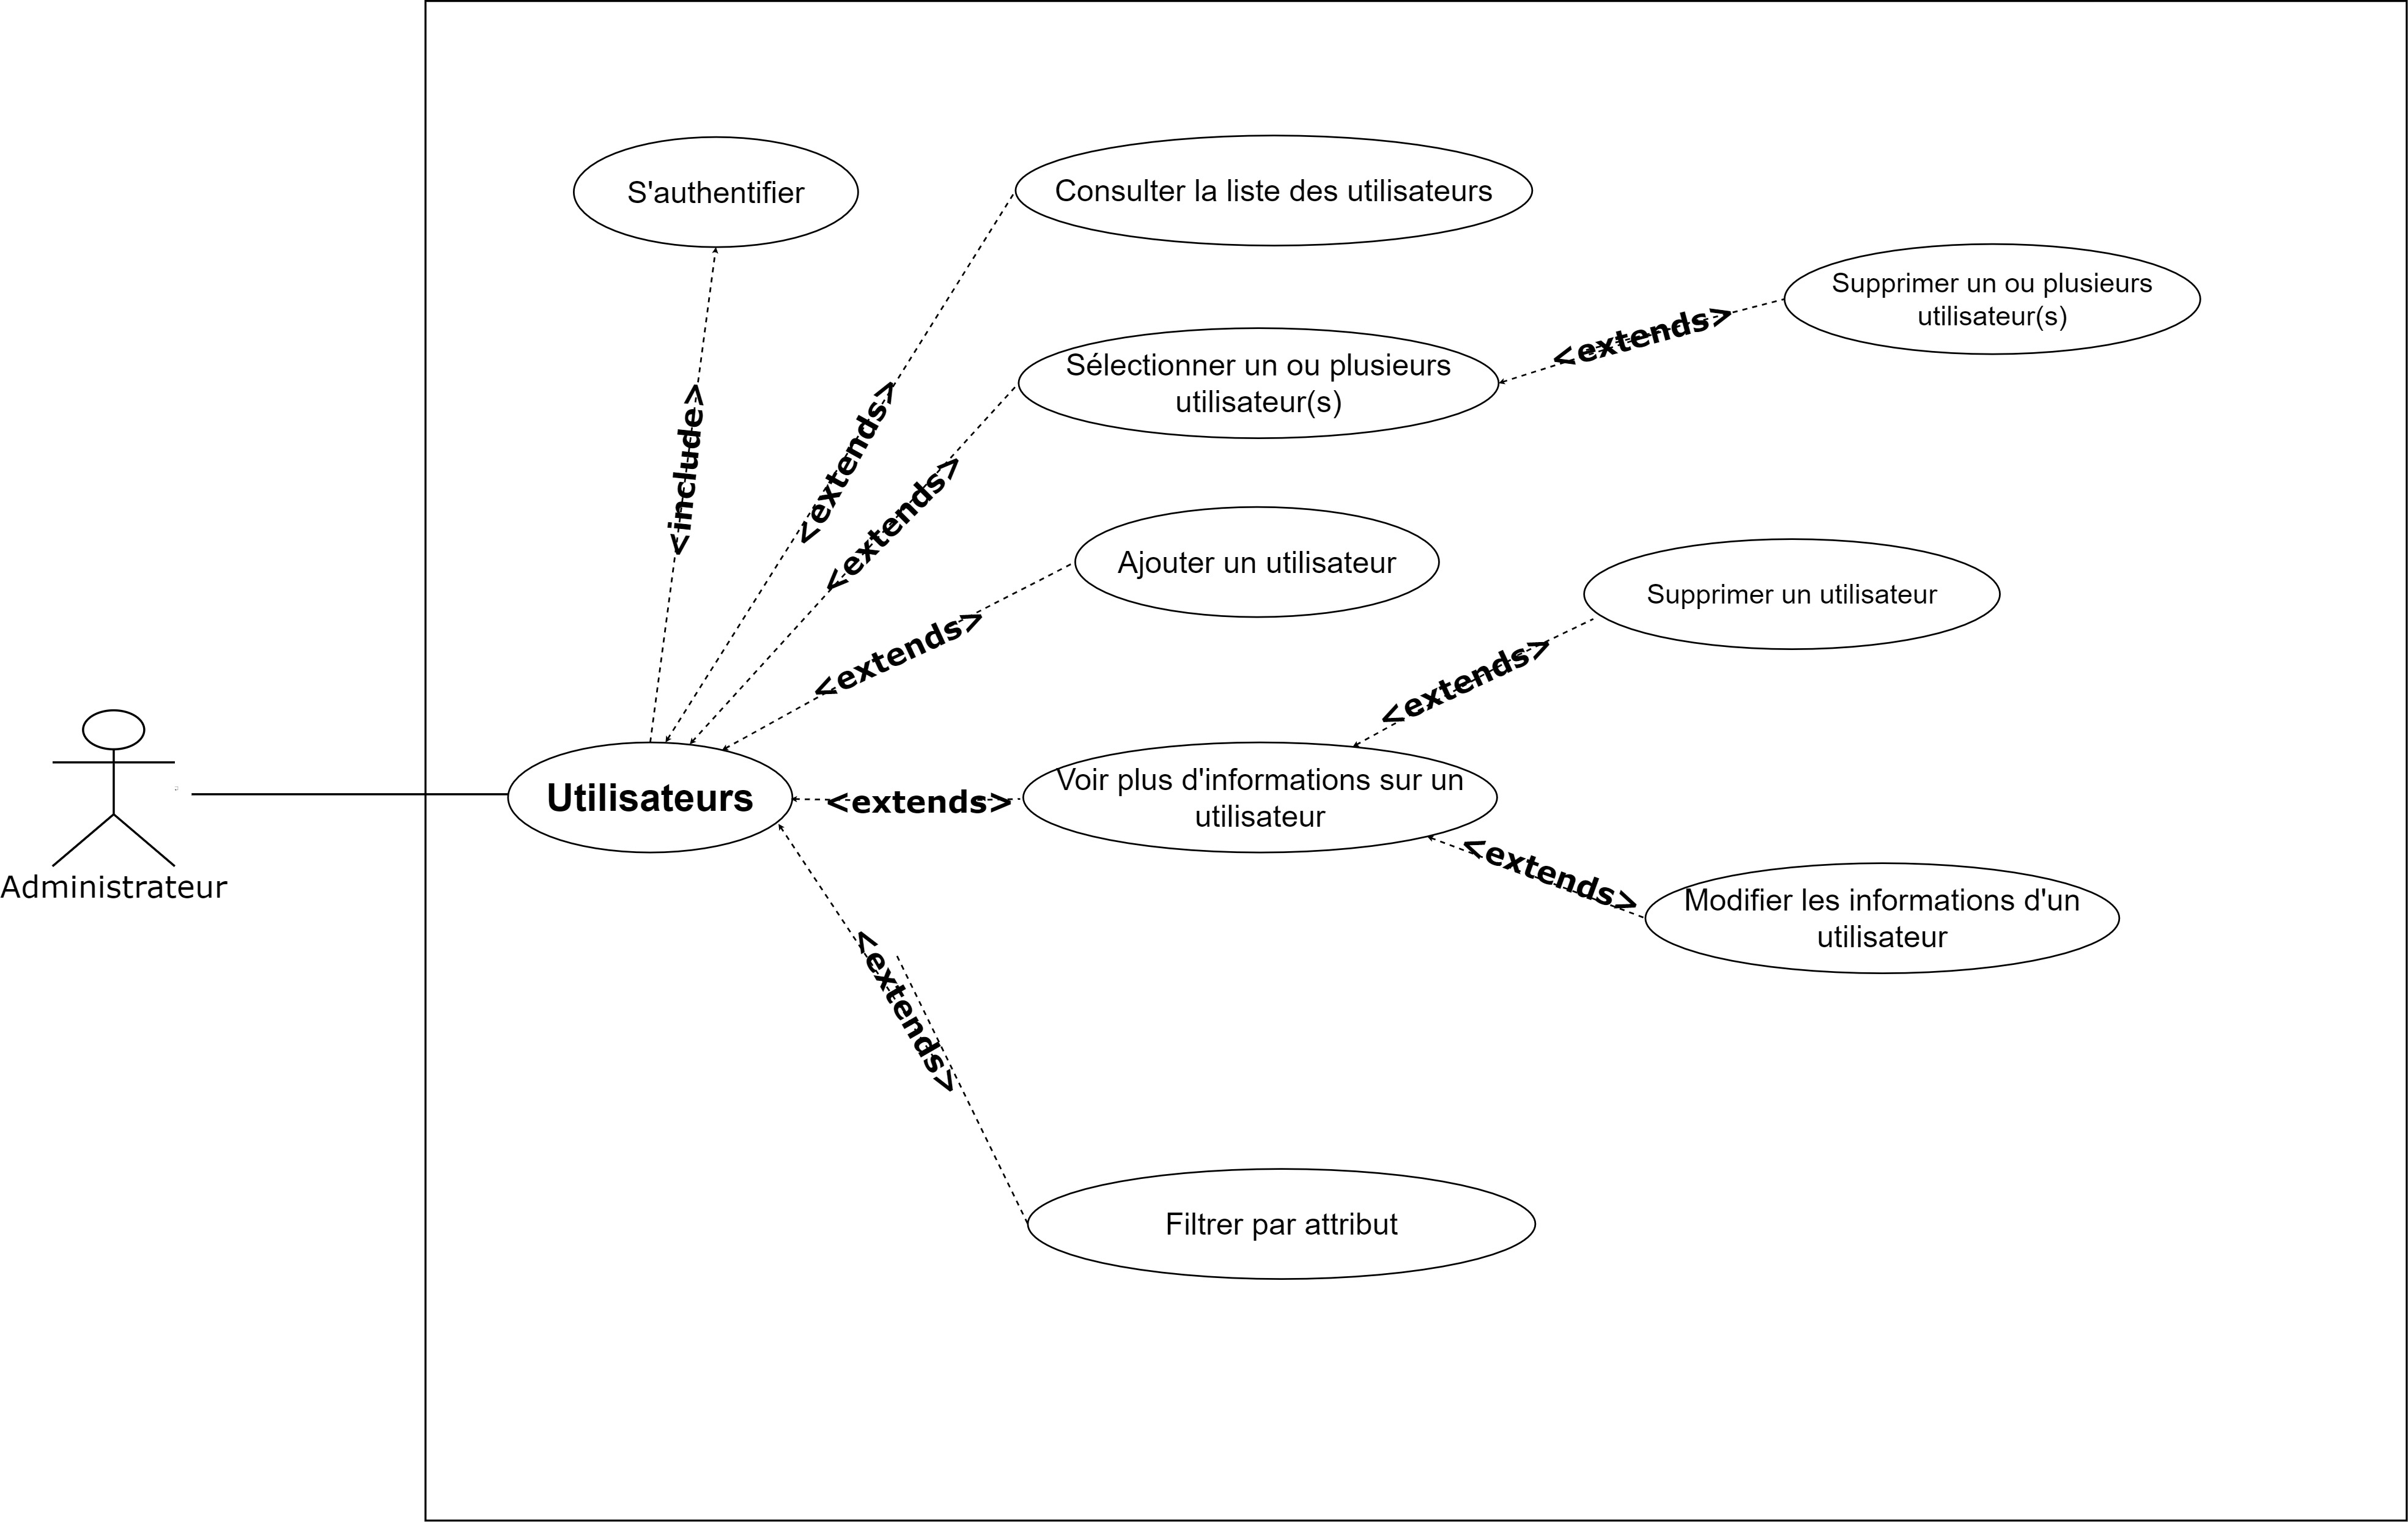
\includegraphics[scale=0.1]{ACR/Diagrammes/Utilisateurs.jpg}
    \caption{Cas d'utilisation 'Utilisateurs'}
\end{figure}


\section{Conception}
Après avoir terminé la modélisation de notre application avec différents diagrammes, nous allons passer à la phase de conception.\\

Nous commencerons par quels que diagrammes de séquence, puis passerons aux diagrammes de classes. Nous finirons avec une présentation de la structure globale de la base de données.\\

\subsubsection{Les diagrammes de séquence}
Les diagrammes de séquence permettent de décrire les scénarios de chaque cas d'utilisation avec une chronologie des opérations.

\paragraph*{Remarque} En vue du nombre important des cas d'utilisation de notre application, nous n'allons présenter que quelques diagrammes de séquences.\\

\textbf{Diagramme de séquence 'Ajout d'un Bus'}
\begin{figure}[H]
    \centering
    \includegraphics[scale=0.55]{ACR/Diagrammes/Séquence ajout bus.jpg}
    \caption{Diagramme de séquence 'Ajout d'un Bus'}
\end{figure}

\textbf{Diagramme de séquence 'Ajout d'un Campus ou d'une Résidence'}
\begin{figure}[H]
    \centering
    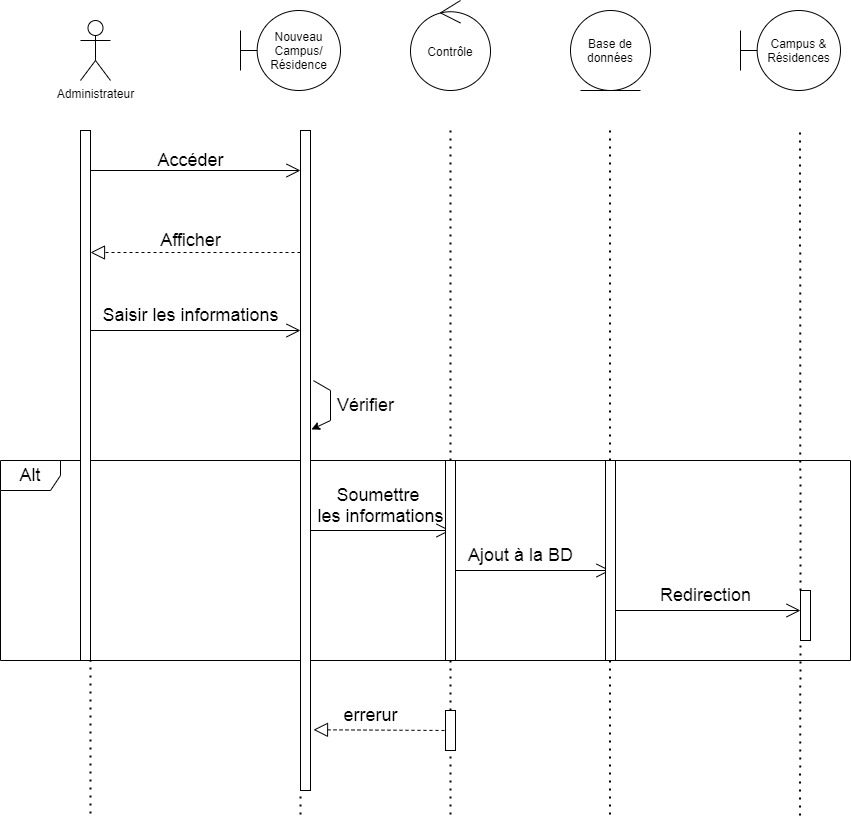
\includegraphics[scale=0.55]{ACR/Diagrammes/Séquence Ajout campus&résidence.jpg}
    \caption{Diagramme de séquence 'Ajout d'un Campus ou d'une Résidence'}
\end{figure}

\textbf{Diagramme de séquence 'Ajout d'un Menu'}
\begin{figure}[H]
    \centering
    \includegraphics[scale=0.55]{ACR/Diagrammes/Séquence ajout menu.jpg}
    \caption{Diagramme de séquence 'Ajout d'un Menu'}
\end{figure}

\textbf{Diagramme de séquence 'Ajout d'un Utilisateur'}
\begin{figure}[H]
    \centering
    \includegraphics[scale=0.55]{ACR/Diagrammes/Séquence Ajout utilisateur.jpg}
    \caption{Diagramme de séquence 'Ajout d'un Utilisateur'}
\end{figure}

\subsubsection{Le diagramme de classe}
Dans la programmation orientée objet, le diagramme de classes est le plus important. Il est le seul obligatoire dans une telle modélisation\\

Le diagramme de classes a pour but de montrer la structure interne du système. Il nous permet d'avoir une vue statique et abstraite de l'ensemble des interactions des objets du système.\\

\paragraph*{Remarque} Pour le pas encombré notre diagramme de classes nous allons définir nos classes, leurs attributs et leurs méthodes d'abord. Par la suite nous définirons les associations et les relations entre les classes.\\

\begin{table}[H]
    \begin{center}
        \begin{tabular}{|Z{5cm}|}
            \hline
            \textbf{Menus}\\
            \hline
            \begin{itemize}
                \item id\_menu
                \item id\_plat\_un
                \item id\_plat\_deux
                \item id\_dessert\_un
                \item id\_dessert\_deux
                \item start
                \item end
                \item recurring
                \item until
                \item interval
                \item freq
                \item title
                \item id\_restaurant
            \end{itemize}\\
            \hline
            \begin{itemize}
                \item[+] Consulter la liste des menus()
                \item[+] Ajouter un menu()
                \item[+] Modifier un menu()
                \item[+] Supprimer un menu()
            \end{itemize}
            \\
            \hline
        \end{tabular}	
        \caption{Classe Menus}
    \end{center}
\end{table}

\begin{table}[H]
    \begin{center}
        \begin{tabular}{|Z{5cm}|}
            \hline
            \textbf{Dossiers de bourse}\\
            \hline
            \begin{itemize}
                \item id\_dossier\_b
                \item nom
                \item prenom
                \item n\_etudiant
                \item n\_tel
                \item email
                \item photo\_id
                \item demande\_b\_sign
                \item attestation\_bac
                \item cert\_scolarite
                \item ext\_naissance
                \item accepted
                \item date\_depot
                \item ext\_role\_impo\_pere
                \item ext\_role\_impo\_mere
                \item ext\_role\_impo\_etud
                \item just\_rev\_pere
                \item just\_rev\_mere
                \item spec\_cheq
            \end{itemize}\\
            \hline
            \begin{itemize}
                \item[+] Consulter la liste des dossiers de bourse()
                \item[+] Consulter les détails d'un seul dossier de bourse()
                \item[+] Ajouter un dossiers de bourse()
                \item[+] Valider un dossiers de bourse()
                \item[+] Refuser un dossiers de bourse()
            \end{itemize}
            \\
            \hline
        \end{tabular}	
        \caption{Classe Dossiers de bourse}
    \end{center}
\end{table}

\begin{table}[H]
    \begin{center}
        \begin{tabular}{|Z{5cm}|}
            \hline
            \textbf{Utilisateurs}\\
            \hline
            \begin{itemize}
                \item id\_user
                \item email
                \item password
                \item displayName
                \item role
            \end{itemize}\\
            \hline
            \begin{itemize}
                \item[+] Consulter la liste des utilisateurs()
                \item[+] Consulter les détails d'un seul utilisateur() 
                \item[+] Ajouter un utilisateur()
                \item[+] modifier un utilisateur()
                \item[+] supprimer un utilisateur()
            \end{itemize}
            \\
            \hline
        \end{tabular}	
        \caption{Classe Utilisateurs}
    \end{center}
\end{table}

\begin{table}[H]
    \begin{center}
        \begin{tabular}{|Z{5cm}|}
            \hline
            \textbf{Trajets}\\
            \hline
            \begin{itemize}
                \item id\_trajet
                \item id\_bus
                \item start
                \item end
                \item recurring
                \item until
                \item interval
                \item freq
                \item title
            \end{itemize}\\
            \hline
            \begin{itemize}
                \item[+] Consulter la liste des trajets()
                \item[+] Consulter les détails d'un seul trajet() 
                \item[+] Ajouter un trajet()
                \item[+] modifier un trajet()
                \item[+] supprimer un trajet()
            \end{itemize}
            \\
            \hline
        \end{tabular}	
        \caption{Classe Trajets}
    \end{center}
\end{table}

\begin{table}[H]
    \begin{center}
        \begin{tabular}{|Z{5cm}|}
            \hline
            \textbf{Bus}\\
            \hline
            \begin{itemize}
                \item id\_bus
                \item matricule
                \item adr\_depart
                \item adr\_arrivee
                \item actif
            \end{itemize}\\
            \hline
            \begin{itemize}
                \item[+] Consulter la liste des bus()
                \item[+] Ajouter un bus()
                \item[+] modifier un bus()
                \item[+] supprimer un bus()
            \end{itemize}
            \\
            \hline
        \end{tabular}	
        \caption{Classe Bus}
    \end{center}
\end{table}

\begin{table}[H]
    \begin{center}
        \begin{tabular}{|Z{5cm}|}
            \hline
            \textbf{Campus et Résidence}\\
            \hline
            \begin{itemize}
                \item id\_camp\_res
                \item nom
                \item adresse
                \item nbr\_lits
            \end{itemize}\\
            \hline
            \begin{itemize}
                \item[+] Consulter la liste des campus et des résidences()
                \item[+] Ajouter un campus ou une résidence()
                \item[+] modifier un campus ou une résidence()
                \item[+] supprimer un campus ou une résidence()
            \end{itemize}
            \\
            \hline
        \end{tabular}	
        \caption{Classe Campus et Résidence}
    \end{center}
\end{table}

\begin{table}[H]
    \begin{center}
        \begin{tabular}{|Z{5cm}|}
            \hline
            \textbf{Dossiers d'Hébergement}\\
            \hline
            \begin{itemize}
                \item id\_dossier
                \item nom
                \item prenom
                \item n\_etudiant
                \item n\_tel
                \item email
                \item photo\_id
                \item demande\_sign
                \item attestation\_bac
                \item cert\_scolarite
                \item cert\_residence
                \item ext\_naissance
                \item accepted
                \item archived
                \item date\_depot
                \item selected\_res
            \end{itemize}\\
            \hline
            \begin{itemize}
                \item[+] Consulter la liste des dossiers d'hébergement()
                \item[+] Ajouter un dossier d'hébergement()
                \item[+] Valider un dossier d'hébergement()
                \item[+] Refuser un dossier d'hébergement()
            \end{itemize}
            \\
            \hline
        \end{tabular}	
        \caption{Classe Dossiers d'Hébergement}
    \end{center}
\end{table}

\begin{table}[H]
    \begin{center}
        \begin{tabular}{|Z{5cm}|}
            \hline
            \textbf{Réstaurants}\\
            \hline
            \begin{itemize}
                \item id\_restaurant
                \item id\_camp\_res
                \item nom
            \end{itemize}\\
            \hline
            \begin{itemize}
                \item[+] Consulter la liste des réstaurants()
                \item[+] Ajouter un réstaurant()
                \item[+] Modifier un réstaurant()
                \item[+] Supprimer un réstaurant()
            \end{itemize}
            \\
            \hline
        \end{tabular}	
        \caption{Classe Réstaurants}
    \end{center}
\end{table}

\begin{table}[H]
    \begin{center}
        \begin{tabular}{|Z{5cm}|}
            \hline
            \textbf{Desserts}\\
            \hline
            \begin{itemize}
                \item id\_dessert
                \item nom
                \item prix
                \item qte\_stock
                \item description
            \end{itemize}\\
            \hline
            \begin{itemize}
                \item[+] Consulter la liste des desserts()
                \item[+] Ajouter un dessert()
                \item[+] Modifier un dessert()
                \item[+] Supprimer un dessert()
            \end{itemize}
            \\
            \hline
        \end{tabular}	
        \caption{Classe Desserts}
    \end{center}
\end{table}

\begin{table}[H]
    \begin{center}
        \begin{tabular}{|Z{5cm}|}
            \hline
            \textbf{Plats}\\
            \hline
            \begin{itemize}
                \item id\_plat
                \item nom
                \item description
            \end{itemize}\\
            \hline
            \begin{itemize}
                \item[+] Consulter la liste des plats()
                \item[+] Ajouter un plat()
                \item[+] Modifier un plat()
                \item[+] Supprimer un plat()
            \end{itemize}
            \\
            \hline
        \end{tabular}	
        \caption{Classe Plats}
    \end{center}
\end{table}

\begin{table}[H]
    \begin{center}
        \begin{tabular}{|Z{5cm}|}
            \hline
            \textbf{Contient}\\
            \hline
            \begin{itemize}
                \item quantite
            \end{itemize}\\
            \hline
        \end{tabular}	
        \caption{Classe Ingrédients d'un Plat}
    \end{center}
\end{table}

\begin{table}[H]
    \begin{center}
        \begin{tabular}{|Z{5cm}|}
            \hline
            \textbf{Ingrédients}\\
            \hline
            \begin{itemize}
                \item id\_ingredient
                \item nom
                \item prix
                \item qte\_stock
            \end{itemize}\\
            \hline
            \begin{itemize}
                \item[+] Consulter la liste des ingrédients()
                \item[+] Ajouter un ingredient()
                \item[+] Modifier un ingredient()
                \item[+] Supprimer un ingredient()
            \end{itemize}
            \\
            \hline
        \end{tabular}	
        \caption{Classe Ingrédients}
    \end{center}
\end{table}


\begin{figure}[H]
    \centering
    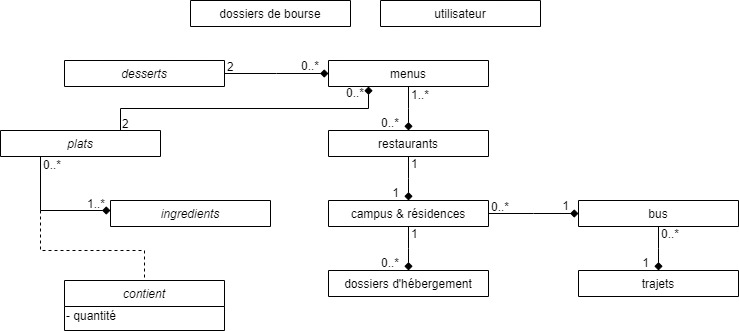
\includegraphics[scale=0.55]{ACR/Diagrammes/class.jpg}
    \caption{Diagramme de classe}
\end{figure}

\subsubsection{Structure de la base de données}
\begin{figure}[H]
    \centering
    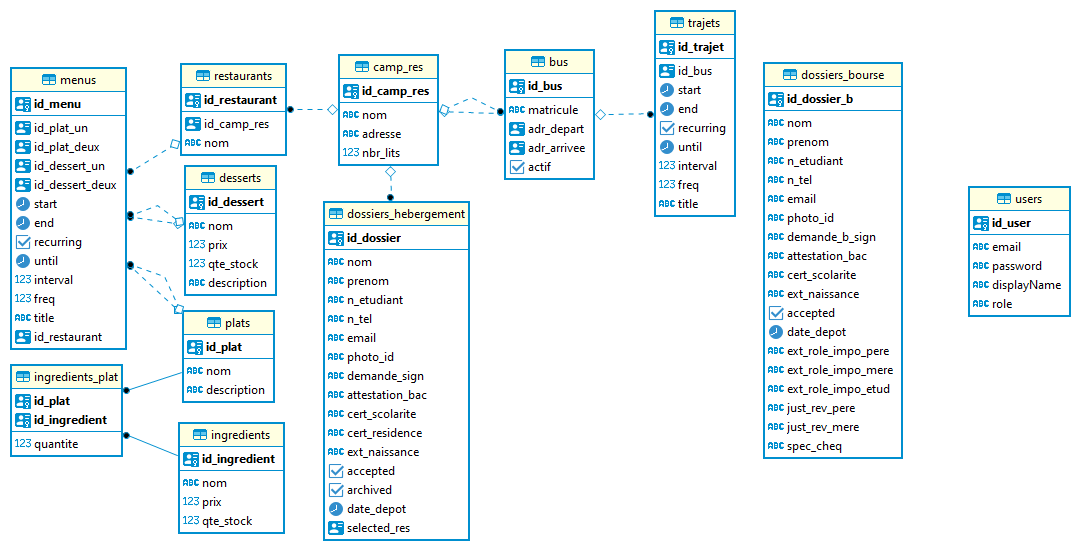
\includegraphics[scale=0.38]{ACR/Diagrammes/diag.png}
    \caption{Structure de la base de données}
\end{figure}

\section{Conclusion}
À l'aide de l'analyse et de la conception, nous avons établi une description graphique de notre projet à travers une utilisation d'\acs{UML} et de ses diagrammes.\\

Nous avons commencé par une présentation et une définition d'\acs{UML} et de ses différents diagrammes.\\

Par la suite, dans la partie analysée, nous avons spécifié les besoins fonctionnels et non fonctionnels de notre application. Ceci nous a mené à l'identification des différents acteurs qui interagissent avec notre système et la spécification des taches de chacun d'eux, ainsi qu'une représentation dès les multiples cas d'utilisation de notre application\\

Finalement, nous sommes passé à la partie conception, où nous avons présenté les différents scénarios du système à l'aide des diagrammes de séquence. Nous avons aussi présenté la structure interne du système à l'aide des diagrammes de classes ainsi qu'une présentation globale de la structure de la base de données.\\

Après avoir analysé et conceptualiser notre système nous allons passer à la partie suite qui est la réalisation de l'application.